\documentclass{article}
\usepackage[utf8]{inputenc}

% math packages
\usepackage{amsmath}
\usepackage{amssymb}
\usepackage{amsthm}
\usepackage{bm}

% bibliography package
\usepackage[round]{natbib}
\bibliographystyle{unsrtnat}
\usepackage{url}

% figures
\usepackage{graphicx}
% \graphicspath{{./figures/}}
\usepackage{caption}
\usepackage{subcaption}

\usepackage{xcolor}
\usepackage{hyperref}

% letter enumerate, enumerate spacing
\usepackage{enumitem}

% nice indicator function
\usepackage{dsfont}

\newtheorem{theorem}{Theorem}[section]
\newtheorem{lemma}[theorem]{Lemma}
\newtheorem{proposition}[theorem]{Proposition}
\newtheorem{remark}{Remark}

\newcommand{\ddt}{\frac{d}{dt}}
\newcommand{\ddtn}[1]{\frac{d^{#1}}{dt^{#1}}}
\newcommand{\todo}{{\color{red} \textbf{TODO} }}
\newcommand{\tXt}{\Tilde{X}_t}
\newcommand{\fle}{\frac{\lambda}{\epsilon}}

\newcommand{\bX}{\mathbf{X}}
\newcommand{\Xt}{\mathbf{X}_t}
\newcommand{\Xj}{\mathbf{X}_j}
\newcommand{\vj}{\mathbf{v}_j}
\newcommand{\R}{\mathbb{R}}
\newcommand{\Rp}{\mathbb{R}^p}

\newcommand{\Ct}{\mathcal{C}_{t}}

\newcommand{\ind}[1]{\mathds{1} \{ #1 \} }
\newcommand{\indep}{\perp \!\!\! \perp}

\DeclareMathOperator*{\argmin}{arg\,min}


\newcommand{\note}[1]{\textcolor{red}{\textit{#1}}}


\title{Caliper Synthetic Matching: Radius Matching with Local Synthetic Controls}
\author{Jonathan Che}
\date{December 2021}

\begin{document}

\maketitle

\begin{abstract}
    Matching promises transparent causal inferences for observational data, making it an intuitive approach for many applications.
    In practice, however, standard matching methods often perform poorly compared to modern approaches such as response-surface modeling and balancing.
    We propose Caliper Synthetic Matching (CSM) to address these challenges while preserving simple and transparent matches and match diagnostics.
    CSM extends Coarsened Exact Matching \citep[CEM; ][]{iacus2012causal} by incorporating general distance metrics, adaptive calipers, and locally constructed synthetic controls.
    We show that CSM can be viewed as a monotonic imbalance bounding (MIB) matching method, so that it inherits and improves upon the usual bounds on imbalance and bias enjoyed by MIB methods.
    Using a simulation study, we illustrate how CSM can outperform modern matching methods in certain settings, and finally illustrate its use on \note{[two real datasets]}.
\end{abstract}

\section{Introduction}

Matching provides a simple approach for drawing causal conclusions from observational data.
In a basic setting, matching methods pair each treated unit with a similar control unit, producing a matched control sample that mirrors the treated sample in terms of observable covariates.
Under standard assumptions, the samples may then be analyzed as if treatment were randomly assigned.
% TODO: above sentence is imprecise
The simplicity of this approach has led matching to be used in a wide range of fields, from aaa to zzz (CITE).
\note{(Can perhaps just remove this paragraph entirely?)}

The gold standard of matching methods is exact matching.
For each treated unit, exact matching finds a control unit with the same observed covariates.
Exact matching therefore perfectly balances the joint covariate distribution between the treated and matched control units,
eliminating any potential bias due to associations between observable covariates and potential outcomes \citep{imai2008misunderstandings}.
Exact matching also produces highly transparent matched datasets,
since the difference in outcomes between a treated unit and its exactly matched control is an unbiased, albeit noisy, estimate of the treatment effect for that treated unit.
This leads to the familiar statistical notion of averaging noisy observations to better estimate a target estimand, e.g., the average treatment effect among all (or some subset) of the treated units.

In practice, however, exact matching is impossible.
Researchers have therefore developed a variety of methods for conducting principled causal inference without exact joint covariate balance.
For example, in practice, standard matching approaches aim for balance on the marginal distributions.
Researchers construct a matched dataset, check the marginal means of the matched sets, and repeat this process if the means are too different (CITE).
Balancing approaches (e.g., CITE a bunch, including Eli and Jose's ``Balancing act in causal inference'' paper) improve on this ad-hoc procedure by directly targeting approximate balance on specified features of the joint distribution.
Semiparametric modeling approaches, such as doubly robust (CITE a bunch), double machine learning (CITE a bunch), and outcome modeling methods (CITE a bunch), use model-assisted averages to target the estimand of interest, leading to provably efficient and unbiased estimates if the models perform reasonably well (CITE).

These modern methods produce effective causal estimates by targeting overall objectives across all units, such as overall covariate balance or good model fit.
In doing so, however, they lose many of the simple intuitions underlying exact matching.
In this paper, we build on a body of literature that focuses on the original spirit of exact matching.
We provide four opinionated maxims for methods in this literature: 
\begin{enumerate}[itemsep=0pt, topsep=12pt, partopsep=0pt]
    \item Distances should be intuitive
    \item Matches should be local
    \item Avoid ``unknown unknowns''
    \item Estimates should be transparent
\end{enumerate}
and we directly construct Caliper Synthetic Matching (CSM) to effectively and clearly address each of these ideas.

CSM may be viewed as an extension to Coarsened Exact Matching \citep[CEM; ][]{iacus2012causal}, a popular method that first coarsens continuous covariates (e.g., splitting an age covariate into four buckets: 0-25, 25-50, 50-75, 75+) before exactly matching observations on their coarsened covariates.
As a result, CSM inherits and improves upon the Monotonic Imbalance Bounding \citep[MIB; ][]{iacus2011multivariate} properties of CEM while preserving its simplicity and intuitiveness.

The rest of the paper proceeds as follows...
Via simulation and real data applications, we show that CSM can exhibit comparable performance to modern methods in various settings while maintaining the intuitive transparency of exact-matching-based methods.

\section{Background}

\subsection{Setup}

Suppose we have $n$ independent and identically distributed observations, with $n_t$ treated units and $n_c$ control units.
For each unit $i$, let $Z_i \in \{0,1\}$ denote its binary treatment status, $Y_i \in \mathbb{R}$ denote its observed real-valued outcome, and $\mathbf{X}_i \equiv \{X_{1i}, \dots, X_{pi} \}^T \in \mathbb{R}^p$ denote its $p$-dimensional real-valued covariate vector.
We use the potential outcomes framework (CITE) and denote the observed outcome for unit $i$ as $Y_i \equiv (1-Z_i) Y_i(0) + Z_i Y_i(1)$, for potential outcomes $Y_i(1)$ and $Y_i(0)$ under the stable unit treatment value assumption (CITE).
We make the standard conditional ignorability assumption:
\begin{align*}
    (Y(1), Y(0)) \indep Z \mid \bX,
\end{align*}
so that conditioning on the observed covariates is sufficient to identify the causal effect of $Z$.
Under a population sampling framework, we write $\epsilon_i \equiv Y_i(Z_i) - f_{Z_i}(\bX_i)$, where $f_0(\bX) \equiv E[Y(0) | \bX]$ and $f_1(\cdot) \equiv E[Y(1) | \bX]$ are the true conditional expectation functions of the potential outcomes under control and treatment, respectively.
We write the set of all treated units' indices as $\mathcal{T} = \{i: Z_i=1\}$, the set of all control units' indices as $\mathcal{C} = \{i: Z_i=0\}$, and the set of the indices of the control units matched to treated unit $t$ as $\Ct = \{i: \text{ unit } i \text{ is matched to unit } t\}$.
Finally, we denote the size of a set $\mathcal{S}$ as $|\mathcal{S}|$.

In this paper, we will focus on estimating the sample average treatment effect on the treated (SATT):
\begin{align*}
    \tau = \frac{1}{n_t} \sum_{j \in \mathcal{T}} Y_j(1) - Y_j(0).
\end{align*}
Under a population sampling framework, the SATT approaches the overall population average treatment effect on the treated (PATT) as the number of treated units increases.
While matching methods can easily be extended to estimate sample and population average treatment effects (SATEs and PATEs), we focus on the SATT to clarify key ideas and simplify exposition.

% Note that we assume continuous covariates $X$.
% We'll assume that we're exactly matching on categoricals we'd like to exact match on.
% If we have an ordinal, we can code it as integers if we're happy to do so; otherwise, we can exact match on those too.


\subsection{Motivation: the spirit of exact matching}
\label{sec:toy}

To motivate the importance of locality and joint balance, we provide a pair of toy examples.
Figure \ref{fig:toy} plots the covariates $X_1$ and $X_2$ of control units $c_i$ and treated units $t_j$.
The colors and contours visualize $f_0(\cdot)$, which takes on greater values in orange within the innermost contour.
To conduct causal inference, we hope to use the observed outcomes of the control units $c_i$ to impute the unobserved counterfactual outcomes of the treated units $t_j$.
\begin{figure}[t]
    \centering
    \begin{subfigure}[ht]{0.4\textwidth}
         \centering
         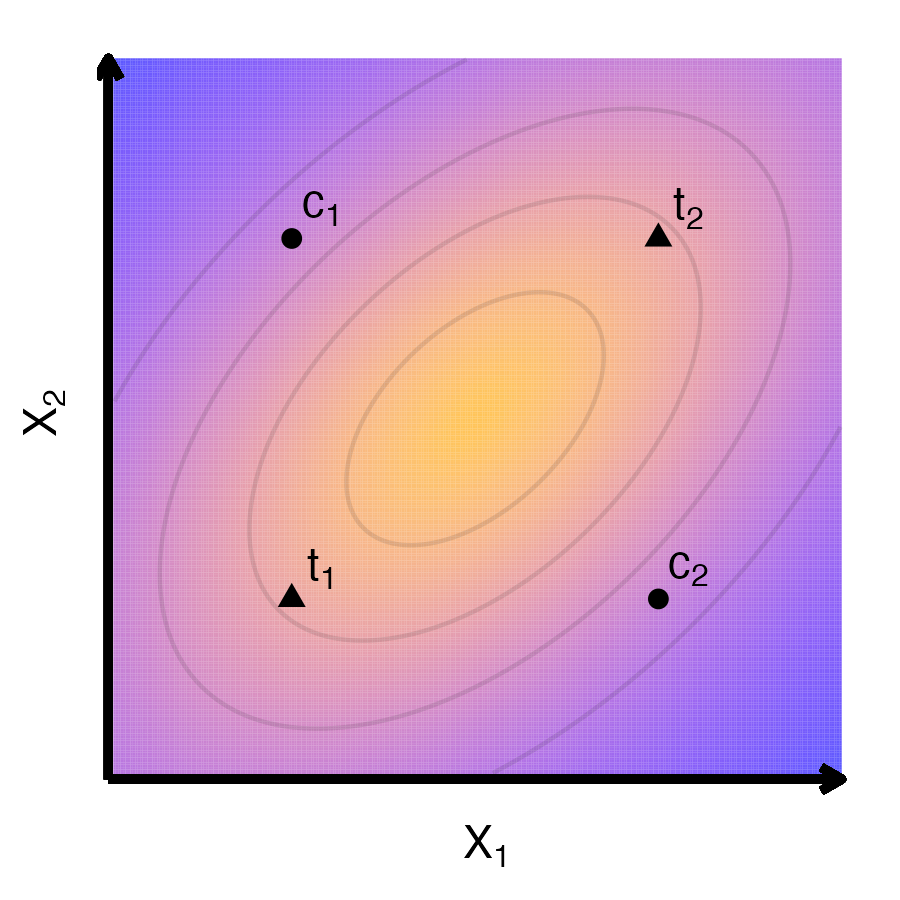
\includegraphics[width=\textwidth]{writeup/figures/toyexample1.png}
         \caption{Toy Example 1}
         \label{fig:toy1}
     \end{subfigure}
     \hspace{5mm}
     \begin{subfigure}[ht]{0.4\textwidth}
         \centering
         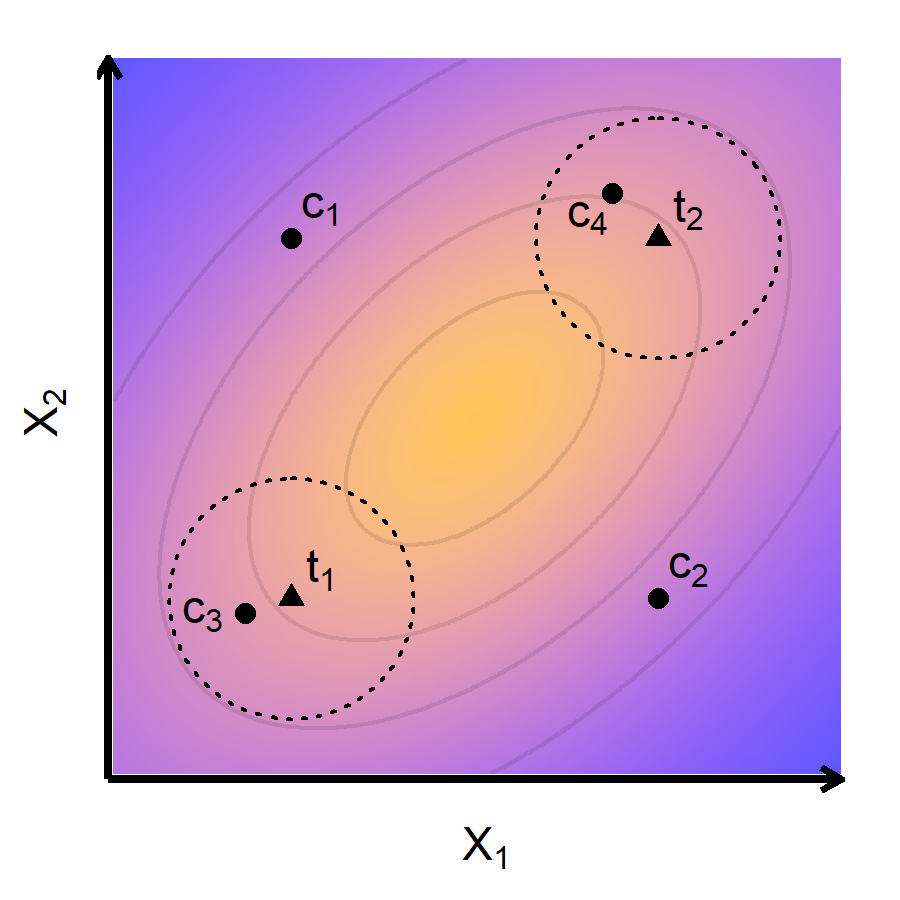
\includegraphics[width=\textwidth]{writeup/figures/toyexample2.png}
         \caption{Toy Example 2}
         \label{fig:toy2}
     \end{subfigure}
    \caption{Toy examples demonstrating utility of locality and joint balance.}
    \label{fig:toy}
\end{figure}

Example 1 (Figure \ref{fig:toy1}) illustrates the dangers of ``unknown unknowns.''
In Example 1, accurate causal inference is not possible due to a lack of overlap; we cannot accurately impute outcomes for $t_1$ and $t_2$ because we do not observe any nearby evaluations of $f_0(\cdot)$.
Many causal inference methods, however, would fail to acknowledge this problem.
For example, a matching or balancing approach may exactly balance both $X_1$ and $X_2$ by assigning weights of 1 to all four units.
Similarly, an outcome model may fit a flat response surface to the observed outcomes of $c_1$ and $c_2$.
Because the usual marginal balance checks and outcome models appear good, the analyst is left unaware that these analyses significantly underestimate counterfactual outcomes, i.e., overestimate the SATT.
Of course, approximate exact matching would also fail here, as there are no control units close to the treated units.
Failing to find local matches, however, alerts the analyst to ``known unknowns,'' i.e., a lack of overlap which indicates potential extrapolation biases.

Example 2 (Figure \ref{fig:toy2}) highlights the role of transparent local matches.
Because $f_0(\cdot)$ is smooth, using only the outcomes of local control units (i.e., controls $c_3$ and $c_4$ within the dotted circles) to impute counterfactual outcomes leads to accurate estimates.
Local matches also produce transparent estimates;
unlike using a black-box outcome model, it is immediately clear how each of the control units contribute to the estimates of each treated unit's counterfactual outcome.
Finally, local matches encourage joint balance.
In Example 2, assigning weights of 1 to $c_1$ and $c_2$ again leads to perfect marginal balance in $X_1$ and $X_2$.
Clearly, however, it is worth sacrificing some marginal balance to upweight $c_3$ and $c_4$, since doing so greatly improves joint balance and downstream estimates.

% Example 2 (Figure \ref{fig:toy2}) highlights the role of joint covariate balance.
% As humans, we cannot visually assess joint balance in more than a few dimensions, so we turn to low-dimensional summaries, e.g., marginal means, to build intuition.
% % While these low-dimensional summaries help identify significant departures from joint covariate balance, they cannot confirm when joint balance is approximately achieved.
% Placing too much emphasis on particular low-dimensional summaries, however, may hurt the resulting causal inferences.
% In Example 2, assigning weights of 1 to $c_1$ and $c_2$ again leads to perfect marginal balance in $X_1$ and $X_2$.
% Clearly, however, it is worth sacrificing some marginal balance to place significantly more weight on $c_3$ and $c_4$, since doing so greatly improves joint balance.

These toy examples illustrate how following ``the spirit of exact matching'' by finding local matches can help both improve causal estimates and diagnose when they may be biased.
In some situations, focusing on joint balance in this way is unnecessary or even harmful;
for example, if the conditional expectation function is additive in its covariates, i.e., $f_0(\bX) = \sum_{j=1}^p g_j(X_j)$ for functions $g_j(\cdot):\mathbb{R} \to \mathbb{R}$, marginal balance suffices (CITE Jose's paper).
In such settings, attempting to balance the full joint covariate distribution is excessively conservative, as it protects estimates from bias that does not exist (e.g., bias due to imbalances in all covariate interactions).

Observational causal inference, however, is often conducted in settings where little is known or assumed about $f_0(\cdot)$, and there are many covariates which may interact with each other in unknown ways.
The toy examples illustrate how, in these settings, leveraging local matches protects analyses against bias that may be otherwise difficult to detect or diagnose.


\note{TODO: figure out how to include the following sentences.
As humans, we cannot visually assess joint balance in more than a few dimensions, so we turn to low-dimensional summaries, e.g., marginal means, to build intuition.
While these low-dimensional summaries help identify significant departures from joint covariate balance, they cannot confirm when joint balance is approximately achieved.
Overemphasizing particular low-dimensional summaries, however, may hurt the resulting causal inferences.
}

\note{TODO: figure out how to add ``minimax'' intuition: by focusing on joint balance we're minimizing the worst-case bias}


% From \href{https://arxiv.org/pdf/2110.14831.pdf}{The Balancing Act in Causal Inference (Ben-Michael et al. 2021)}:
% ``We need balance in the mean outcome conditional on treatment and covariates for IPW,
% and in the errors we make when estimating it for AIPW.
% This happens when we estimate the inverse propensity weights and this conditional mean function sufficiently well...''
% Specifically:
% \begin{align*}
%     \hat{\mu}_1 - \mu_1 = \frac{1}{n} \sum \frac{W_i}{\hat{e}(X_i)} m_1(X_i) - \frac{1}{n} \sum m_1(X_i) + irreducible noise/sampling error
% \end{align*}
% and for AIPW, replace $m_1(\cdot)$ with $\hat{m}_1(\cdot) - m_1(\cdot)$.
% RESPONSE: The idea we're getting at is:
% if we really don't know the conditional expectation function (slash it's hard to estimate),
% we need to be conservative here;
% as such, approximately balancing the joint distributions serves as a sufficient conditional for approximately balancing the $m_1(\cdot)$.
% In general, outcome models aren't very transparent about where they're less certain, and it's hard to back this out, particularly in moderate dimensions.

\note{TODO: see what balancing does when we're just given control units everywhere, and treated units only in certain places.}


\subsection{Related work}
\label{sec:related}

TODO: some sort of ``family tree'' or a chronology of methods.
Like exact matching $\implies$ CEM, propensity score matching and diagnostics $\implies$ balancing approaches, etc.?

Matching methods have a long history in observational causal inference (CITE Rosenbaum, Imbens and Rubin, etc).
Rather than attempt an exhaustive review, we briefly trace how these methods have operationalized the spirit of exact matching over time and then provide more detailed surveys in Section \ref{sec:CSM} as we develop the method introduced in this paper.

Early work in matching incorporated locality via nearest-neighbor (CITE), caliper (CITE), and radius matching (CITE) approaches.
These methods were typically combined with dimension reduction, e.g., via propensity scores (CITE), to circumvent the challenge of near-exact matching with multiple covariates,
though some approaches, e.g., Mahalanobis distance matching (CITE), directly operated on a scaled version of the original covariate space.
To evaluate their matched sets, researchers would typically conduct iterative balance checks, revising their matching scheme if it led to poor marginal mean balance (CITE?)

To circumvent the need for these iterative balance checks, \citet{iacus2012causal} introduced Coarsened Exact Matching (CEM), which we discuss in further detail in Section \ref{sec:close}.
Instead of fixing the sample and returning the resulting level of balance, CEM fixes a user-specified level of joint balance and returns the resulting sample.
By making local matches a primary rather than a secondary criterion, CEM enjoys the desirable transparency and joint balance properties of exact matching.

In recent years, significant work has been developed in the field of ``almost-exact'' matching, which attempts to more precisely (or exactly) match covariates that appear to be more predictive of the potential outcomes.
\citet{dieng2019interpretable} and \citet{wang2021flame} do so for discrete covariates, and \citet{morucci2020adaptive} and \citet{parikh2022malts} extend this work to continuous covariates.
% TODO: cite Eli's balancing act to note that all that needs to be balanced is the conditional expectation function.

Recent work outside of matching has also noted the importance of locality in observational causal inference.
\citet{abadie2021penalized} augments the popular synthetic controls methodology with a penalty for using units far from the treated unit.
In a similar synthetic controls setting, \citet{ben2021augmented} tunes extrapolation away from the convex hull of control units.
\citet{kellogg2021combining} explicitly trades off bias due to extrapolating beyond local matches with bias due to linearly interpolating between distant units.
\note{TODO: other papers to note?}

\note{Writeup also mentions \href{https://scholar.google.com/scholar?q=raking+survey+sampling&hl=en&as_sdt=0&as_vis=1&oi=scholart}{raking} (i.e., finding weights that balance marginals in survey samples) within calipers, though this is closer to balancing than to matching.}
\note{Writeup also suggests possibly using kernel approaches within calipers, which I should mention somewhere.}


\section{Caliper Synthetic Matching}
\label{sec:CSM}

\citet{stuart2010matching} decomposes matching analyses into two phases.
In the design phase, researchers select a distance measure, use it to run a matching method, and diagnose the quality of the resulting matches.
In the subsequent analysis phase, researchers use the matched units to estimate treatment effects.
% We highlight a key principle from each of these steps and construct our proposed matching method to satisfy these principles while preserving transparency and interpretability.

In this section, we propose a matching method that satisfies key principles from each of these four stages.
We construct our method in a modular fashion;
at each stage, we increase the complexity of the method to improve its use of the data.
While we believe that the final proposed method simultaneously maximizes transparency and performance, in practice researchers may make different choices at each stage to limit complexity as necessary.

\subsection{Principle 1: Distances should be intuitive}

In the absence of exact matches, matching algorithms find control units as ``close'' as possible to their treated counterparts to improve joint covariate balance and reduce potential bias \citep{rosenbaum1985bias}.
For matching, one popular distance measure is propensity score distance:
\begin{align}
\label{eq:ps}
    d^{(e)}(\bX_i, \bX_j) = |e(\bX_i) - e(\bX_j)|,
\end{align}
where the propensity score $e(\cdot) = P(Z_i = 1 \mid \bX_i)$ represents the probability that a unit is treated, given its covariates \citep{rosenbaum1983central}.

While matching units with similar propensity scores leads to principled causal estimates, it does not construct intuitive matched sets.
Propensity score distance is not formally a distance metric on $\mathbb{R}^p$,\footnote{For example, $d^{(e)}(\bX_i, \bX_j) = 0$ does not imply that $\bX_i = \bX_j$.
For a simple introduction to distance metrics on $\mathbb{R}^p$, see Appendix \ref{app:biasbd}.}
so it can violate our natural understanding of ``closeness.''
For example, two units that are ``close'' in terms of propensity score distance may have very different covariate values.
If a researcher matches two such units, it can be unclear whether they should trust this match, fit a better propensity-score model, or find a closer propensity-score match.
% While propensity scores are useful in many causal inference settings, using them for matching can lead to counterintuitive results \citep{king2019propensity}.

Formal distance metrics provide a more natural approach for assessing similarity between units.
Researchers are generally familiar with the covariates in their data, 
so directly attaching a distance metric to the space of covariates builds upon existing intuitions.
Multidimensional distance metrics typically take the form of a scaled Euclidean (i.e., $L_2$) distance metric:
\begin{align}
\label{eq:l2dist}
    d^{(2)}_V(\bX_i, \bX_j) = \sqrt{(\bX_i - \bX_j)^T (V^T V) (\bX_i - \bX_j)}
\end{align}
or scaled $L_\infty$ distance metric:
\begin{align}
\label{eq:linfdist}
    d^{(\infty)}_V(\bX_i, \bX_j) 
    %= ||V (\bX_i - \bX_j)||_\infty 
    = \sup_{k = 1, \dots, p} |V (\bX_i - \bX_j)|_k,
\end{align}
for a given $p \times p$ symmetric positive definite matrix $V$.
The matrix $V$ scales the raw differences in the covariates and their two-way interactions.
For example, if $V_{11}$ were large, then the resulting distance metric would magnify, i.e., upweight, differences in the first covariate.

A variety of scaled distance metrics have been proposed in the literature.
One popular scaled $L_2$ distance metric is Mahalanobis distance, which uses $V^T V = \Sigma^{-1}$, the inverse covariance matrix estimated from the control group (CITE).
Other $L_2$ approaches restrict the scale matrix $V^T V$ to be diagonal and directly optimize it.
To learn optimal covariate weights from the data, genetic matching \citep{diamond2013genetic} optimizes covariate balance, Matching After Learning to Stretch \citep{parikh2022malts} minimizes the resulting predictive error over a hold-out training set, and synthetic controls \citep{abadie2010synthetic} minimize the resulting predictive error across hold-out outcome variables in a time-series setting.

In this paper, we let $V$ be a diagonal matrix implicitly determined by a given covariatewise caliper, as formalized in Proposition \ref{prop:distmetriccal}.
We consider both scaled $L_2$ and scaled $L_\infty$ distance metrics, 
though we note that $L_\infty$ metrics can be particularly intuitive in higher dimensions.
% $L_\infty$ metrics have a natural coordinate-wise interpretation:
% to check whether the distance between two units is less than $\epsilon$ scaled $L_\infty$ units, one may simply check whether the absolute differences in each of their coordinates $j$ is less than $\epsilon V_{jj}$.
Specifically, with $L_\infty$ metrics, coordinates are ``independent'' in the sense that changing any non-maximal absolute difference in coordinates between two units does not affect the $L_\infty$ distance between them.
This is naturally related to the Monotonic Imbalance Bounding \citep[MIB; ][]{iacus2011multivariate} property, which we discuss in Section \ref{sec:mib}.

% Appendix \ref{app:metricchoice} provides further details about how to select an appropriate $V$ matrix.

% https://math.stackexchange.com/questions/1927845/is-u-v-in-the-svd-of-a-symmetric-positive-semidefinite-matrix
% [NOTE: could make $V$ be on the same scale in Equations \ref{eq:l2dist} and \ref{eq:linfdist}.
% E.g., add a square root to Equation \ref{eq:l2dist}; and in Equation \ref{eq:linfdist}, SVD the positive definite $V$ matrix into $V=UDU^T$ and use $V^* = U\sqrt{D}$, the rotation and sqrt of scaling piece.
% This is extra nice because we can say that if $U \neq I$ (e.g., as it does for Mahalanobis distance scaling), the $V^*$ matrix is ``not interpretable.'']

\subsection{Principle 2: Matches should be local}
\label{sec:close}

Given a chosen measure of ``closeness,'' there are many ways to select the closest matched units.
One popular approach is nearest-neighbors matching, where each treated unit is matched with the control unit(s) closest to it.
This can be done either greedily for each treated unit \citep{rubin1973matching} or optimally over all treated units \citep{rosenbaum1989optimal}.
Nearest-neighbors matching is also commonly conducted after some preprocessing steps, such as learning an optimal distance metric \citep{diamond2013genetic, parikh2022malts}.

While nearest-neighbors approaches are intuitive, they can quietly fail to achieve covariate balance.
While nearest-neighbors approaches guarantee that each treated unit is matched with its closest controls, the closest controls may still be quite far.
Large distances between treated units and their matched controls, i.e., low match quality, can lead to poor joint covariate balance.

To combat this problem, many methods apply calipers coupled with nearest-neighbor matching.
Calipers are a distance $c$ beyond which matches are forbidden.\footnote{Calipers modify the distance metric as:
\begin{align*}
    d(\bX_i, \bX_j) = 
    \begin{cases}
        d(\bX_i, \bX_j) &\text{if } d(\bX_i, \bX_j) \leq c \\
        \infty &\text{if } d(\bX_i, \bX_j) > c
    \end{cases}
\end{align*}}
Using calipers, nearest-neighbor approaches can avoid problems associated with poor match quality, using the closest matches only if they are ``close enough.''

In this paper, we directly use all control units within a given $L_\infty$-norm caliper of each treated unit, maximizing the number of local matches used to produce causal estimates.
This is known as radius matching \citep{dehejia2002propensity}, though previous proposals used propensity score distances.
We relegate discussion of caliper selection to Appendix \ref{app:caliperchoice}.

Using all units within a given $L_\infty$-norm caliper has strong connections to coarsened exact matching (CEM) \citep{iacus2012causal}.
% a method that has seen significant use in applied settings due to its ease of interpretation and implementation.
In CEM, continuous variables are first coarsened into discrete bins, e.g., an age variable may be coarsened into the bins 0-25, 25-50, 50-75, and 75-100.
Observations are then exactly matched on their coarsened covariates.
% CEM therefore preserves the spirit of exact matching, making it feasible by doing so on coarsened covariates.
Using $L_\infty$ calipers generalizes this idea of exact matching on coarsened covariates, as we discuss in further detail in Section \ref{sec:compCEM}.

% Figure [TODO] compares CEM to $L_\infty$ calipers using a toy example with two continuous covariates.
% The CEM coarsening implicitly defines calipers shown by the dashed gridlines, where each cell contains units that are exactly matched on the coarsened covariates.
% For example, the two treated units in the top-left cell are matched (with replacement) with the three control units in that cell, and the treated unit in the bottom-right cell has no matches, so it gets dropped from the data.
% Given any covariate coarsening, we can define an $L_\infty$ caliper of the same size, shown by the solid boxes.\footnote{One attractive feature of CEM is the option to use unevenly sized coarsenings, e.g., age into the bins 0-25, 25-40, 40-60, and 60+.
% We discuss how to do this with $L_\infty$ calipers in TODO.
% IDEA: we avoid non-translation-invariant distance metrics, since they are hard to understand.
% We can directly transform the data to get at the idea that 0-10k is the same as 10k-100k, e.g., log10!}
% Though the caliper remains the same size, we now see that the treated unit in the bottom-right cell can be matched with the nearby control unit on the other side of the coarsened gridline.
% Centering calipers on each treated unit rather than in the center of the coarsened grid allows us to better capture all of the control units ``close enough'' to each treated unit.
% Doing so also preserves the spirit of exact matching; 
% we exactly match control units not to the treated units themselves, but rather to the neighborhoods of the treated units as defined by their calipers.

\subsection{Principle 3: Avoid ``unknown unknowns''}
% \subsection{Principle 3: Matches should be easy to assess}

An important step in any matching procedure is to assess the resulting matches.
Marginal balance checks may reveal significant departures from joint balance but cannot confirm when joint balance is approximately achieved, as demonstrated in Toy Examples 1 and 2.
Checking low-dimensional summaries of joint balance also fails to assess overlap or identify subsets of the treated units for which it may be easier or more difficult to estimate treatment effects, leaving room for potential ``unknown unknowns.''

% Using a distance-metric caliper, on the other hand, directly ensures approximate joint covariate balance.
% Though some covariate imbalance naturally remains after caliper matching, it is clearly controlled (e.g., see Proposition \ref{prop:wass}).
% As a result, the potential imbalance-induced bias is well-characterized, as discussed in \citet{iacus2011multivariate} and elaborated upon in Section \ref{sec:biasbd}.

Using a distance-metric caliper, on the other hand, directly ensures good covariate balance (e.g., see Proposition \ref{prop:wass}), so practitioners no longer need to assess it \citep{iacus2012causal}.
The resulting loss of data, however, can significantly change the target estimand.
Calipers identify treated units that do not have close matches, i.e., the treated units that have poor overlap with the control units.
Dropping these difficult-to-match units improves the quality of the resulting estimate but changes the estimand from the SATT to the feasible sample average treatment effect (FSATT):
$$\tau_\mathcal{F} = \frac{1}{|\mathcal{F}|} \sum_{t \in \mathcal{F}} Y_t(1) - Y_t(0),$$
where $\mathcal{F}$ denotes the set of indices of treated units with at least one control unit within $c$ $d_V^{(\infty)}$ units, i.e., $\mathcal{F} = \{t \in \mathcal{T}: \exists \ j \in \mathcal{C} \text{ with } d_V^{(\infty)}(\Xt, \Xj) \leq c\}$.

To target the SATT, we assign each treated unit $t$ an adaptive caliper $c_t$.
We let $c_t = \max \{c, d_t\}$, where $c$ is a global caliper and $d_t = \min_{j:Z_j=0} d(\bX_t, \bX_j)$ is the distance between unit $t$ and its nearest control-unit neighbor \citep{dehejia2002propensity}.
In data-rich contexts, the adaptive caliper may also be selected so that the resulting matched sets work well with synthetic controls (introduced in the following section), e.g., by letting $c_t$ be the smallest caliper such that treated unit $t$ has $p+1$ within-caliper controls.

Adaptive calipers ensure that every treated unit receives at least one match, allowing the resulting estimate to target the SATT.
The wider calipers, however, lead to lower-quality estimates.
We use the calipers $c_t$ across all treated units to assess this estimate-estimand tradeoff,
creating balance-sample-size frontier plots \citep{king2017balance} to show how dropping poorly matched treated units affects both potential bias and the SATT estimate for the remaining sample.
We also summarize characteristics of units with different $c_t$ values to better understand regions with poorer overlap.\footnote{See Section \ref{sec:lalonde} for an example of these assessments on the Lalonde dataset \citep{lalonde1986evaluating}.}
Overall, rather than using diagnostic plots to attempt to assess joint balance using low-dimensional summaries, we use them to clearly characterize the estimate-estimand tradeoff, allowing researchers to qualitatively assess the potential bias they are willing to accept to estimate the SATT.

% [Random idea:
% for $C$ the region of $\mathbb{R}^p$ covered by the caliper of width $c$ and $dens(\cdot)$ some density estimator of the control units:
% \begin{align*}
%     \min_c \int_C 1 - \lambda dens(x) dx
% \end{align*}
% We want to minimize caliper size (first term) and maximize the density covered by the caliper (second term), with tradeoff dictated by $\lambda$.]

\subsection{Principle 4: Estimates should be transparent}

Given matched units from the design phase of a matching analysis, the final step is to produce an estimate.
With high-quality matches, the SATT may be estimated with a simple average:
$$\hat{\tau}^{avg} = \frac{1}{n_t} \sum_{t \in \mathcal{T}} \big( Y_t - \frac{1}{|\Ct|} \sum_{j \in \Ct} Y_j \big).$$
Typically, however, researchers apply outcome models, e.g., weighted linear regression, to the matched dataset to adjust for residual covariate imbalances (CITE).

In this paper, we use the synthetic control method \citep[SCM; ][]{abadie2010synthetic} within matched sets.
For each treated unit $t$, we find convex weights for its matched control units that minimize covariate imbalance as measured by a scald distance metric $d_V(\cdot, \cdot) = d_V^{(2)}(\cdot, \cdot)$ or $d_V^{(\infty)}(\cdot, \cdot)$:
\begin{align*}
    \argmin_{\{w_{jt} : j \in \Ct\}} 
        &\hspace{2mm} d_V(\Xt, \sum_{j \in \Ct}w_{jt} \Xj) \\
    \text{s.t. } 
        &\sum_{j \in \Ct} w_{jt} = 1 \\
        &0 \leq w_{jt} \leq 1 \text{ for } j \in \mathcal{C}_t,
\end{align*}
where we've written the weight for control unit $j$ associated with treated unit $t$ as $w_{jt}$.
The ``synthetic control'' unit for treated unit $t$ gets covariates $\sum_{j \in \Ct}w_{jt} \Xj$ and outcome $\sum_{j \in \Ct}w_{jt} Y_j$,
and the ATT estimate is taken as a simple difference-in-means between the outcomes of the treated units and their synthetic controls:
\begin{align*}
    \hat{\tau}_t^{SC} = \frac{1}{n_t} \sum_{t \in \mathcal{T}} \big(Y_t - \sum_{j \in \Ct} w_{jt} Y_j \big).
\end{align*}

The setup above deviates from the standard SCM setup in a few ways.
First, while \citet{abadie2010synthetic} introduces SCM as a quadratic programming problem using scaled $L_2$ distance, we also allow SCM to be implemented as a linear programming problem using scaled $L_\infty$ distance (see Appendix \ref{app:scm} for details).
Second, while synthetic controls are typically used in time-series settings with past outcomes as additional covariates, we directly apply them in our setting without past outcomes.
Finally, the SCM introduced in \citet{abadie2010synthetic} includes an outer optimization to learn an ``optimal'' scaling matrix $V$, whereas we simply use the $V$ matrix implied by the given covariatewise caliper (as formalized in Proposition \ref{prop:distmetriccal}).

\note{TODO: within-caliper extrapolation?}

Using synthetic controls in the analysis phase provides two primary benefits.
First, synthetic controls are highly transparent.
Because synthetic controls explicitly produce a counterfactual for each treated unit, researchers can directly check whether each counterfactual seems reasonable.
Second, synthetic controls naturally reduce bias within calipers.
Synthetic controls are mathematically equivalent to linear interpolation.\footnote{See Appendix \ref{app:scm} for details.}
While linear interpolation over long distances can lead to bias, interpolating over short distances, such as within a caliper, typically improves results due to the local linearity of smooth outcome functions, as we discuss in Section \ref{sec:biasbdscm}

We denote the use of synthetic controls within adaptive $L_\infty$ calipers Caliper Synthetic Matching (CSM).
As previously discussed, CSM uses a scaled $L_\infty$ distance for its simplicity and its connections to exact matching.
Adapting the caliper enables clear diagnostic plots of the estimate-estimand tradeoff and synthetic controls produce interpretable local bias corrections.

\section{Properties}
\label{sec:properties}
\subsection{Monotonic Imbalance Bounding}
\label{sec:mib}

\citet{iacus2011multivariate} introduces the Monotonic Imbalance Bounding (MIB) class of matching methods.
MIB matching methods directly control covariate balance between the treated and matched control groups, independently for each covariate.\footnote{Technically, \cite{iacus2011multivariate} defines the MIB property with respect to a particular function of the data and a particular discrepancy measure.
In the manuscript, however, the authors casually describe methods as MIB if they are MIB with respect to all covariatewise absolute differences between matched units.
We use this convention here and relegate further discussion of technical details to Appendix \ref{app:mib}.}
As a result, MIB matching methods enjoy desirable properties such as bounded covariate imbalance and bounded estimation error, under reasonable assumptions.

Distance-metric caliper matching methods are MIB as long as the caliper for each covariate may be tuned without affecting the caliper for any other covariate \citep{iacus2011multivariate}.
Any such covariatewise caliper can be satisfied by a scalar caliper on an appropriately scaled distance metric.
For example, if $p=2$ and we want to ensure $|X_{t1} - X_{j1}| \leq 2$ and $|X_{t2} - X_{j2}| \leq 5$, we may define $V = \begin{bmatrix} \frac{1}{2} & 0 \\ 0 & \frac{1}{5} \end{bmatrix}$ so that restricting $d^{(\infty)}_V(\Xt, \Xj) \leq 1$ satisfies the desired caliper.
This idea is formalized by Proposition \ref{prop:distmetriccal}.
\begin{proposition}
\label{prop:distmetriccal}
    Given covariatewise caliper $\boldsymbol{\pi} \in \mathbb{R}^p_{+}$ on units $t$ and $j$, for scaling matrix $V = diag\{\frac{1}{\boldsymbol{\pi}}\}$:
    \begin{enumerate}[label=(\alph*)]
        \item $d^{(2)}_V(\Xt, \Xj) \leq 1 \implies |X_{tk}-X_{jk}| \leq \pi_k \text{ for } k=1,\dots,p $
        \label{prop:dmca}
        \item $ d^{(\infty)}_V(\Xt, \Xj) \leq 1 \iff |X_{tk}-X_{jk}| \leq \pi_k \text{ for } k=1,\dots,p $
        \label{prop:dmcb}
    \end{enumerate}
\end{proposition}
\begin{proof}
    \begin{enumerate}[label=(\alph*)]
        \item Without loss of generality, suppose for contradiction that $|X_{tk}-X_{jk}| > \pi_k \text{ for } k=1$. 
        Then:
        \begin{align*}
            d^{(2)}_V(\Xt,\Xj) 
            = \sqrt{\sum_{k=1}^p \frac{(X_{tk}-X_{jk})^2}{\pi_k^2}}
            \geq \sqrt{\frac{(X_{t1}-X_{j1})^2}{\pi_1^2}}
            > 1.
        \end{align*}
        \item This follows from definitions:
        \begin{align*}
            d^{(\infty)}_V(\Xt, \Xj) \leq 1
            &\iff \sup_{k = 1, \dots, p} |\frac{X_{tk} - X_{jk}}{\pi_k}| \leq 1 \\
            % &\iff |\frac{X_{tk} - X_{jk}}{\pi_k} \leq 1 \text{ for } k=1,\dots,p \\
            &\iff |X_{tk}-X_{jk}| \leq \pi_k \text{ for } k=1,\dots,p 
        \end{align*}
    \end{enumerate}
\end{proof}
% NOTE: scaling by $\frac{1}{p\pi^2}$ gives the circumscribed circle, scaling by $\frac{1}{\pi^2}$ gives the inscribed circle

Proposition \ref{prop:distmetriccal} shows how any given covariatewise caliper $\boldsymbol{\pi}$ induces a scale $V$ for the distance metric.\footnote{Note that the choice to bound $d^{(2)}_V(\Xt, \Xj)$ and $d^{(\infty)}(\Xt, \Xj)$ by 1 is arbitrary, e.g.,
bounding $d^{(\infty)}_V(\Xt, \Xj) \leq 1$ is equivalent to bounding $d^{(\infty)}_V(\Xt, \Xj) \leq c$ for $c>0$ and $V = diag\{\frac{c}{\pi}\}$.
In Proposition \ref{prop:distmetriccal}, we choose $c=1$ for simplicity.}
Tighter calipers on a covariate imply that distances in that covariate are magnified, i.e., scaled up relative to distances in other covariates.

% \footnote{Note also that Proposition \ref{prop:distmetriccal}\ref{prop:dmcb} is an equivalence, unlike \ref{prop:distmetriccal}\ref{prop:dmca}.
% A covariatewise caliper defines a hyperrectangle around each treated unit, which is equivalent to a scaled $L_\infty$-norm ball but larger than an inscribed scaled $L_2$-norm ball.}

CSM with fixed calipers is a member of the MIB class of matching methods.
With adaptive calipers, CSM is MIB for the feasible treated units within $\mathcal{F}$ but extrapolates for the other treated units,
though the adaptive calipers still provide transparency about the extent to which CSM leaves the MIB class.
In the subsequent sections, we focus on CSM with fixed calipers, restating and clarifying some of the important properties of MIB matching methods.


\subsection{Bounded joint covariate imbalance}

MIB matching methods bound the distance between each treated unit and its matched controls, naturally making the treated and matched-control covariate distributions similar.
This similarity can be quantified in many ways.
For example, \citet{iacus2012causal} shows that CEM bounds the absolute differences between the treated and matched control units' marginal moments and distributions.
% empirical means, marginal centered $k^{\text{th}}$ moments, and marginal quantiles.
% In this section, we show that radius matching with a scaled distance metric also bounds the distance between the marginal empirical means and, more generally, the full empirical joint covariate distributions of the treated and matched control units.

Rather than focusing on marginal balance, we directly show how distance-metric caliper matching methods control joint covariate imbalance.
To do so, we introduce some notation.
Write the empirical joint covariate distributions of the treated and control units as:
\begin{align*}
    f_T(\mathbf{x}) 
    &= \frac{1}{n_T} \sum_{t \in \mathcal{T}} \delta_{\Xt}(\mathbf{x}) \\
    f_C(\mathbf{x}) 
    &= \frac{1}{n_T} \sum_{t \in \mathcal{T}} \sum_{j \in \Ct} w_{jt} \delta_{\Xj} (\mathbf{x}),
\end{align*}
% Write the empirical joint covariate distributions of the treated and control units as:
% \begin{align*}
%     F_T(\mathbf{x}) 
%     &= \frac{1}{n_T} \sum_{t \in \mathcal{T}} \ind{\Xt \preccurlyeq \mathbf{x}} \\
%     F_C(\mathbf{x}) 
%     &= \frac{1}{n_T} \sum_{t \in \mathcal{T}} \sum_{j \in \Ct} w_{jt} \ind{\Xj \preccurlyeq \mathbf{x}},
% \end{align*}
% where $\bX \preccurlyeq \mathbf{x}$ means that $X_k \leq x_k$ for all $k = 1, \dots, p$.
where $\delta_{\bX}(\cdot)$ represents a Dirac delta function at $\bX$, i.e., $\delta_{\bX}(\mathbf{y}) = 1$ if $\mathbf{y} = \mathbf{X}$ and $0$ otherwise.
The empirical distributions are simply weighted sums of point masses located at the matched units' covariates.

To demonstrate how distance-metric calipers control the difference between $f_T$ and $f_C$, we use Wasserstein distance.
Formally, the $q$-Wasserstein distance between probability distributions $P$ and $Q$ with distance metric $d(\cdot, \cdot)$ is:
\begin{align*}
    \mathcal{W}_q(P, Q) = \inf_{\substack{\bX \sim P \\ \mathbf{Y} \sim Q}} E\big[ d(\bX, \mathbf{Y})^q \big]^{1/q},
\end{align*}
where the infimum is over couplings of $P$ and $Q$, i.e., all joint distributions with marginals $P$ and $Q$.
Wasserstein distance is also known as ``earth-mover's distance'':
viewing $P$ and $Q$ as piles of soil each with total mass 1, $W_q(P, Q)$ measures the minimum ``cost'' to move soil to make $P$ match $Q$ (or vice-versa), where the ``cost'' of moving $k$ units of soil from $\mathbf{x}$ to $\mathbf{y}$ is $k\cdot d(\mathbf{x}, \mathbf{y})$.
Wasserstein distance naturally extends distance metrics to measure distance between full probability distributions rather than distances between points.

% Now let $X_1, \dots, X_n \overset{i.i.d.}{\sim} P$ and $Y_1, \dots, Y_n \overset{i.i.d.}{\sim} Q$.
% Then the Wasserstein $p$-distance between the empirical distributions of $P$ and $Q$ may be written as:
% \begin{align*}
%     \mathcal{W}_p(P, Q) = \inf_{\pi} \big( \frac{1}{n} d(X_i, Y_{\pi(i)})^p \big)^{1/p},
% \end{align*}
% where $\pi(\cdot): \{1, \dots, n\} \to \{1, \dots, n\}$ represents a permutation of $n$ elements.

With this notation in hand, Proposition \ref{prop:wass} shows that radius matching bounds the Wasserstein distance between $f_T$ and $f_C$.

\begin{proposition}
\label{prop:wass}
    For caliper $c > 0$ and a given matching method:
    \begin{enumerate}[label=(\alph*)]
        \item For all $t$, $d^{(2)}_V(\Xt, \Xj) \leq c$ for all $j \in \Ct$
            $\implies \mathcal{W}^{(2)}_q(f_T, f_C) \leq c$
        \item For all $t$, $d^{(\infty)}_V(\Xt, \Xj) \leq c$ for all $j \in \Ct$
            $\implies \mathcal{W}^{(\infty)}_q(f_T, f_C) \leq c$
    \end{enumerate}
\end{proposition}
\begin{proof}
    The full proof is given in Appendix Proposition \ref{prop:wass_real}.
    To illustrate the main ideas, let $\bX_t^{(C)} = \sum_{j \in \Ct} w_{jt} \Xj$ denote the weighted sum of the covariates of the control units associated with each treated unit $t$,
    and let $f_C^*$ denote the empirical joint distribution of $\bX_t^{(C)}$ for $t = 1, \dots, n_T$.

    Notably, $f_T$ and $f_C^*$ are each constructed using $n_T$ point masses, one for each treated unit.
    As a result, we may express the $q$-Wasserstein distance between $f_T$ and $f_C^*$ using the distance metric $d^{(\cdot)}_V(\cdot, \cdot)$ as:
    \begin{align*}
        \mathcal{W}^{(\cdot)}_q(f_T, f_C) 
        &= \inf_{\substack{\bX \sim f_T \\ \mathbf{Y} \sim f_C^*}} E\big[ d_V^{(\cdot)}(\bX, \mathbf{Y})^q \big]^{1/q} \\
        &= \inf_{\pi} \Big( \frac{1}{n_T} \sum_{t \in \mathcal{T}} d^{(\cdot)}_V(\bX_t, \bX^{(C)}_{\pi(t)})^q \Big)^{1/q},
    \end{align*}
    where $\pi(\cdot): \{1, \dots, n\} \to \{1, \dots, n\}$ represents a permutation of $n$ elements and the superscript on $\mathcal{W}$ indicates $L_2$ or $L_\infty$ distance.
    This is because the set of couplings of the empirical distributions $f_T$ and $f_C$ is simply equivalent to the set of possible pairings of all of their $n_T$ point masses.
    As a result:
    \begin{align*}
        \mathcal{W}^{(\cdot)}_q(f_T, f_C) &=
        \inf_{\pi} \big( \frac{1}{n_T} \sum_{t \in \mathcal{T}} d^{(\cdot)}_V(\bX_t, \bX^{(C)}_{\pi(t)})^q \big)^{1/q} \\
        &\leq \big( \frac{1}{n_T} \sum_{t \in \mathcal{T}} d^{(\cdot)}_V(\bX_t, \bX^{(C)}_{t})^q \big)^{1/q} 
            &[\text{Choose } \pi(t)=t] \\
        &\leq c.
            &[d^{(\cdot)}_V(\bX_t, \bX^{(C)}_{t}) \leq c]
    \end{align*}
    The last line holds because $d^{(\cdot)}_V(\Xt, \Xj) \leq c$ for all control units $j \in \Ct$, and $\bX_t^{(C)}$ is a convex combination of the control units in $\Ct$.
\end{proof}

We make two remarks about Proposition \ref{prop:wass}.
First, while the notation is technical, the intuition is straightforward.
Distance-metric calipers control how far each treated unit's covariates can be from its matched controls' covariates.
Since $f_T$ and $f_C$ are simply weighted sums of the point masses associated with these covariates, the calipers must also control the distance between $f_T$ and $f_C$.
% For example, consider a treated unit $t$ and its single matched control $j$ such that $d^{(\infty)}_V(\Xt, \Xj) = \epsilon$.
% Then the point mass corresponding to the treated unit's covariates needs to be moved $\epsilon$ $d_V^{(\infty)}$-units to coincide with the point mass corresponding to the control unit's covariates, 
% i.e., $\mathcal{W}_q^{(\infty)}(\delta(\Xt-\mathbf{x}), \delta(\Xj-\mathbf{x})) = d^{(\infty)}_V(\Xt, \Xj) = \epsilon$.
Second, note that for an exact caliper $c=0$, Proposition \ref{prop:wass} simply states that exact matching guarantees that $f_T$ coincides with $f_C$.
In practice, however, reducing the caliper size to $c=0$ drops all of the treated units, leaving the proposition to be vacuously true, so $c$ must be chosen with the estimate-estimand tradeoff in mind.

Control over joint covariate imbalance naturally implies control over marginal imbalances.
For example, Appendix Proposition \ref{prop:meanbd} shows how distance-metric calipers also bound the distance between the empirical weighted covariate means of the treated and matched control units.
In summary, distance-metric calipers enable precise control of joint covariate imbalance.
This leads to a variety of desirable properties illustrated in the following sections.
% Propositions \ref{prop:meanbd} and \ref{prop:wass} demonstrate the utility of caliper-based methods by formalizing their basic intuition:
% if the covariates for each treated unit are required to be similar to the covariates of its matched controls, then the treated and matched control covariate distributions must be close to each other.
% This joint covariate balance may be summarized using the marginal means, or it may be directly demonstrated using Wasserstein distance.


\subsection{Bounded bias}
\label{sec:biasbd}

Because MIB matching methods bound the distance between the covariates of matched units, they naturally bound the distance between smooth functions $f:\mathbb{R}^p \to \mathbb{R}$ of those covariates as well.
Recall that we may write write the control potential outcome for unit $i$ as $Y_i(0) = f_0(\bX_i) + \epsilon_i$.
Then assuming that $f_0(\cdot)$ is smooth (i.e., Lipschitz) immediately bounds the bias of any FSATT estimate produced by a method using distance-metric calipers.
\begin{proposition}
\label{prop:biasbd_lip}
Suppose $f_0: \mathbb{R}^p \to \mathbb{R}$ is Lipschitz$(\lambda)$ with respect to $d_V(\cdot, \cdot)$ = $d^{(2)}_V(\cdot, \cdot)$ or $d^{(\infty)}_V(\cdot, \cdot)$.
Then for a matching procedure such that for all $t$, $d_V(\Xt, \Xj) \leq c$ for all $j \in \Ct$:
\begin{equation*}
    \big|E[\tau_\mathcal{F} - \hat{\tau}_\mathcal{F}] \big| \leq \lambda c.
\end{equation*}
\end{proposition}
\begin{proof}
    \begin{align*}
        \big| E &[\tau_\mathcal{F} - \hat{\tau}_\mathcal{F} ] \big| \\
        &= \bigg| E\Big[\frac{1}{n_T}\sum_{t \in \mathcal{T}} \big( Y_t(1) - Y_t(0) \big) - \frac{1}{n_T}\sum_{t \in \mathcal{T}} \big( Y_t(1) - \sum_{j \in \Ct} w_{jt} Y_j(0) \big) \Big] \bigg| \\
        % &= \bigg| \frac{1}{n_T} \sum_{t \in \mathcal{T}} 
        %     E\Big[ \sum_{j \in \Ct} w_{jt} Y_j(0) - Y_t(0) \Big]\bigg| \\
        &= \bigg| \frac{1}{n_T} \sum_{t \in \mathcal{T}} 
            \Big( \sum_{j \in \Ct} w_{jt} \big(f_0(\Xj) - f_0(\Xt)\big) \Big) \bigg| \\
        &\leq \bigg| \frac{1}{n_T} \sum_{t \in \mathcal{T}} 
            \Big( \sum_{j \in \Ct} w_{jt} \lambda d(\Xj, \Xt) \Big) \bigg| \\
        &\leq \lambda c.
    \end{align*}
\end{proof}

Proposition \ref{prop:biasbd_lip} states that for distance-metric caliper matching methods, worst-case bias is proportional to the caliper size $c$.\footnote{Proposition \ref{prop:biasbd_lip} applies to a slightly different set of methods than Proposition 1 from \citet{iacus2011multivariate}, which proves a similar bias bound for MIB matching methods.}
As in Proposition \ref{prop:wass}, setting $c=0$ shows that exact matching leads to unbiased estimates, but in practice we must use $c > 0$ to navigate the estimate-estimand tradeoff without dropping all of the treated units.

Of course, we rarely know the Lipschitz constant $\lambda$ in practice, so it is difficult to use Proposition \ref{prop:biasbd_lip} to generate empirical bias bounds.
Nonetheless, Proposition \ref{prop:biasbd_lip} illustrates how distance-metric calipers control bias:
If each treated unit is close to all of its matched controls in covariate space, its expected counterfactual outcome must be close to their expected outcomes, for reasonable (i.e., smooth) outcome functions.
As a result, any weighted average of the control units' outcomes cannot differ too much in expectation from the treated unit's true counterfactual outcome, regardless of the specific form of $f_0(\cdot)$.

\subsection{Bias reduction from synthetic controls}
\label{sec:biasbdscm}

% \note{TODO: also worth noting the directional derivative stuff here, how the assumption relates to directional derivatives along paths existing. Luke wants to make the math alive via some intuition.}

While using distance-metric calipers bounds bias, using synthetic controls within these calipers actively reduces bias.
Specifically, synthetic controls naturally remove linear bias by conducting local linear interpolation.\footnote{See Appendix \ref{app:scm} for further details.}
This means that if $f_0(\cdot)$ is linear, exact synthetic controls completely eliminate bias.
Otherwise, bias is controlled by higher-order nonlinear trends in $f_0(\cdot)$, which are less influential within tight calipers.
Proposition \ref{prop:scbiasbd} more precisely shows how exact synthetic controls eliminate linear bias.
\begin{proposition}
\label{prop:scbiasbd}
Let $d_V(\cdot, \cdot)$ = $d^{(2)}_V(\cdot, \cdot)$ or $d^{(\infty)}_V(\cdot, \cdot)$.
Suppose $f_0: \mathbb{R}^p \to \mathbb{R}$ is differentiable and Lipschitz($\lambda$) with respect to $d_V$.
Then for a matching procedure such that for all $t$, $d_V(\Xt, \Xj) \leq c$ for all $j \in \Ct$,
if $\sum_{j \in \Ct} w_{jt} \Xj = \Xt$ for all $t$:
\begin{equation*}
    % |\sum_j w_{jt} f(\Xj) - f(\Xt)| \leq o(c)
    \big|E[\tau - \hat{\tau}] \big| \leq o(c).
\end{equation*}
\end{proposition}
\begin{proof}
    See Appendix \ref{app:biasbd}.
\end{proof}

In Proposition \ref{prop:scbiasbd}, the $o(c)$ term represents higher-order terms which go to zero more quickly than does the caliper $c$ as $c$ shrinks toward zero.
In practice, shrinking $c$ to zero drops all treated units, but the notation highlights how implementing synthetic controls within calipers takes advantage of local linearity:
while linear interpolation of nonlinear functions across large distances can lead to significant interpolation bias \citep{kellogg2021combining},
restricting the donor-pool units to be within a caliper distance from the treated unit reduces the impact of nonlinearities, which play a much smaller role across short distances.

Proving Proposition \ref{prop:scbiasbd} requires some additional mathematical exposition.
Specifically, we require $f_0(\cdot)$ to be differentiable in order to Taylor expand it with respect to the given distance metric.
The resulting expansion differs from the usual multivariate Taylor expansion, since it uses directional derivatives to better utilize the distance-metric calipers.
We provide further details in Appendix \ref{app:biasbd}.


\subsection{Comparison to CEM}
\label{sec:compCEM}

As discussed in Section \ref{sec:close}, radius matching methods have many similarities with coarsened exact matching (CEM) \citep{iacus2012causal}.
Indeed, as an MIB method, CEM possesses the imbalance-bounding and bias-bounding guarantees discussed in the previous sections.

To clarify the benefits of radius matching, Figure \ref{fig:vs_cem} visualizes the CEM caliper grid defined by a uniform coarsening of two covariates, $X_1$ and $X_2$,
along with the equivalently sized $L_\infty$ caliper around treated unit $t_1$.
\begin{figure}
    \centering
    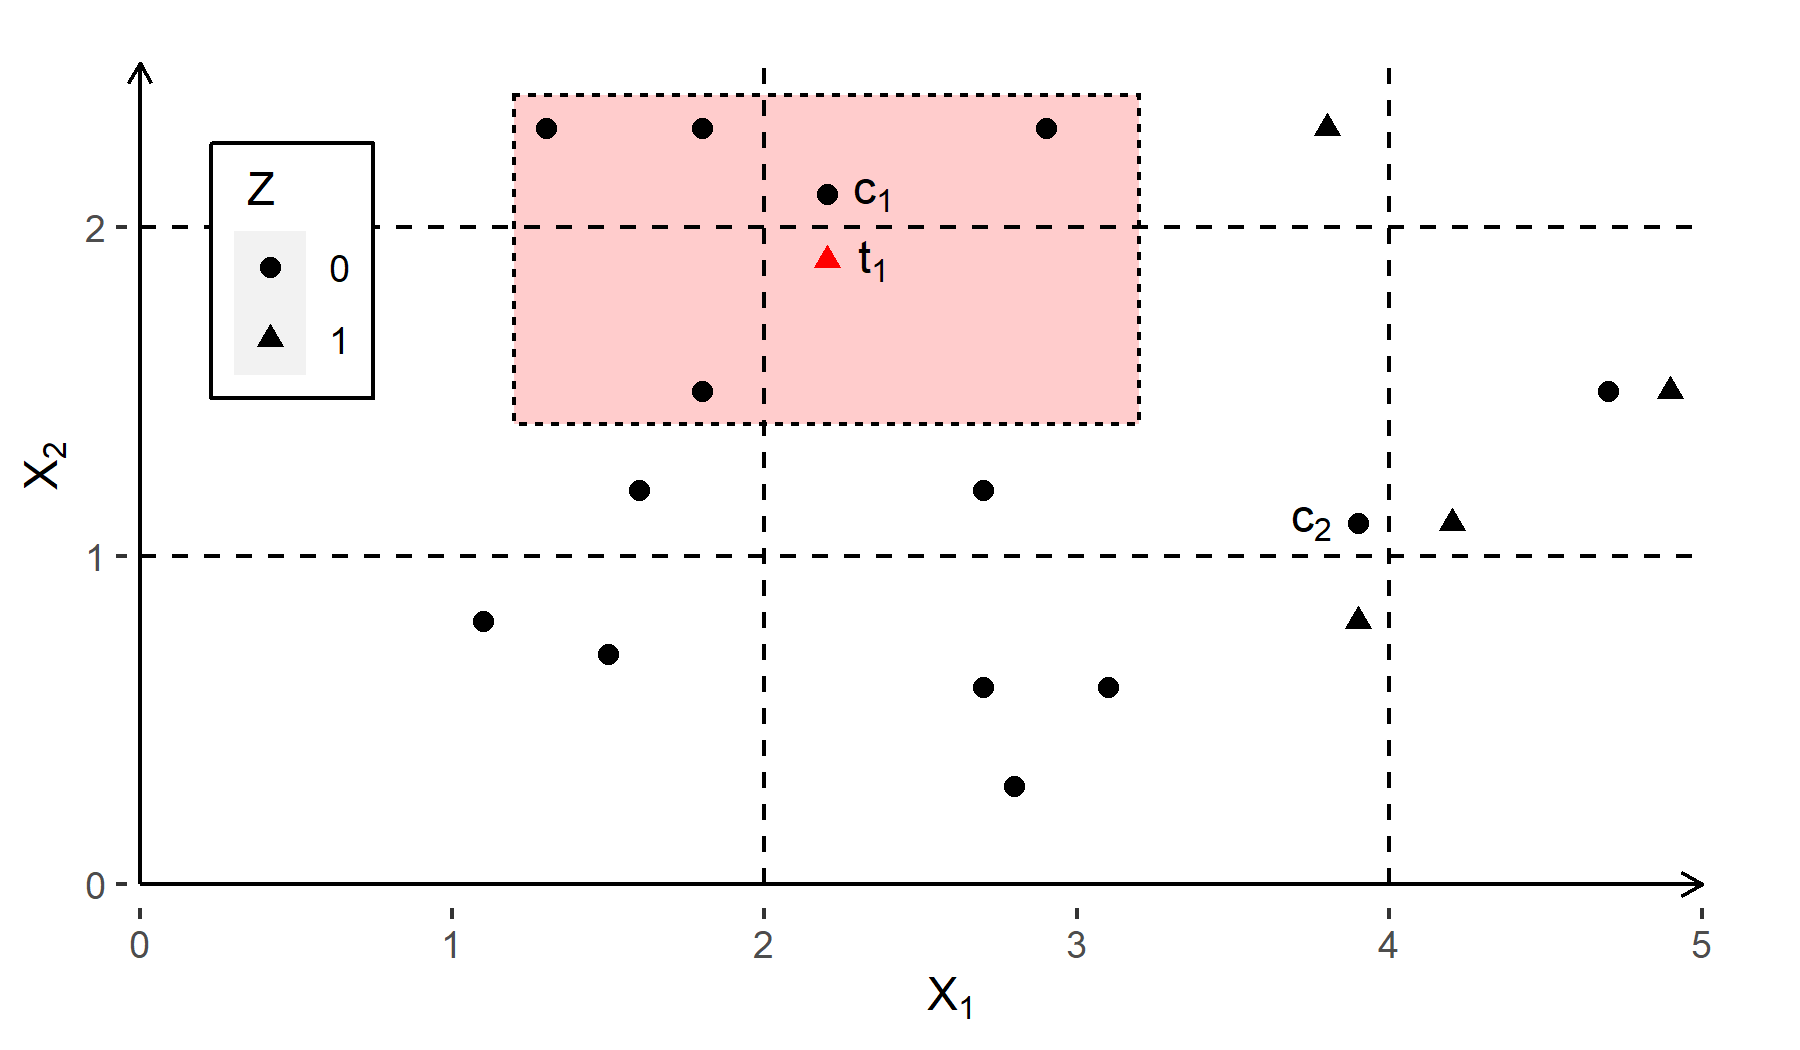
\includegraphics[width=\textwidth]{writeup/figures/show_cem_calipers.png}
    \caption{Comparison of coarsened exact matching with radius matching using $L_\infty$ calipers.
    Dashed gridlines represent CEM calipers.
    Shaded box represents scaled $L_\infty$ caliper around point $t_1$.}
    \label{fig:vs_cem}
\end{figure}
Because $t_1$ lies near a boundary defined by the covariate coarsening, CEM does not match $t_1$ to $c_1$, while the $L_\infty$ caliper does.
On the other hand, CEM matches $t_1$ to $c_2$ because they lie in the same caliper grid, even though the two units lie more than one $L_\infty$ unit apart from each other.
Figure \ref{fig:vs_cem} shows how, given a fixed caliper size, CEM guarantees that treated units lie within two $L_\infty$ units of their matched controls whereas the $L_\infty$ caliper guarantees the distance is no more than one unit.
By centering calipers on each treated unit, radius matching matches each treated unit to all nearby control units while guaranteeing imbalance and bias bounds that are twice as tight as those guaranteed by CEM.

Naturally, there are tradeoffs for these improved bias bounds.
Computationally, radius matching requires computing distances between each treated unit and the control units, an operation of order $n_t n_c$, unlike CEM which only requires a frequency tabulation of order $n_t+n_c$.
Non-uniform calipers are also slightly easier to implement via covariate coarsenings, though we argue that for many common covariates it can be more straightforward to directly transform the covariate and use a uniform caliper rather than attempting to define a non-uniform caliper.\footnote{E.g., rather than non-uniformly coarsening income as \{ \$0-20k, \$20k-50k, \$50k-100k, \$100k+ \}, it may be more reasonable to log-transform the income covariate and use a uniform caliper to avoid, e.g., concluding that an individual earning \$20k is as far from an individual earning \$20.1k as they are from an individual earning \$50k.}
Overall, however, radius matching preserves the transparency and interpretability of CEM while significantly improving on its useful bias and imbalance bounding properties.


\subsection{Bias-variance tradeoff}

Reducing caliper sizes reduces the potential bias of the resulting SATT estimate, as shown by Proposition \ref{prop:biasbd}, but may increase the estimate's variance.
To formalize this idea, we introduce the (conditional) mean-squared error for the SATT $\tau$:
\begin{align*}
    CMSE = E[(\hat{\tau} - \tau)],
\end{align*}
where the expectation is implicitly conditioned on the observed covariates and treatment assignments \citep{kallus2020generalized}.
Standard algebraic manipulation then shows that $CMSE = B^2 + V^2$, for:
\begin{align*}
    B^2 &= 
        \Big(\frac{1}{n_T} \sum_{t \in \mathcal{T}} \sum_{j \in \Ct} 
            w_{jt} \big( f_0(\Xt) - f_0(\Xj) \big) \Big)^2 \\
    V^2 &=
        \frac{1}{n_T^2} \sum_{t \in \mathcal{T}} \sigma_t^2 +
        \frac{1}{n_T^2} \sum_{j \in \mathcal{C}} (\sum_{t \in \mathcal{T}} w_{jt})^2 \sigma_j^2,
\end{align*}
where $\sigma_i$ represents the population sampling variance of unit $i$ conditional on its covariates $\bX_i$.
% Here we allow any weights such that $\sum_{j \in \mathcal{C}} w_{jt} = 1$ for all $t$.
If we assume homoskedasticity (i.e., $\sigma_i = \sigma$) and the conditions of Proposition \ref{prop:biasbd_lip} with caliper $\epsilon$, we can bound CMSE as:
\begin{equation}
\label{eq:cmsebd}
    CMSE \leq 
        (\lambda \epsilon)^2 +
        \frac{\sigma^2}{n_T} \Big(1 + \frac{\sum_{j \in \mathcal{C}} (\sum_{t \in \mathcal{T}} w_{jt})^2}{n_T} \Big).
\end{equation}

Equation \ref{eq:cmsebd} clarifies the relationship between caliper size and the bias-variance tradeoff.
For a fixed estimand,\footnote{I.e., if we do not add or drop treated units as caliper size changes} increasing $\epsilon$ naturally exposes the resulting estimate to more bias.
Increasing $\epsilon$ also generally reduces variance by dispersing weight across more control units, reducing $\sum_{j \in \mathcal{C}} (\sum_{t \in \mathcal{T}} w_{jt})^2$.
Note, however, that variance is typically dominated by the variance associated with the treated units, which remains unchanged as control units are added.\footnote{In most cases, $\sum_{j \in \mathcal{C}} (\sum_{t \in \mathcal{T}} w_{jt})^2 \leq n_T$, since $\sum_{j \in \mathcal{C}} \sum_{t \in \mathcal{T}} w_{jt} = n_T$ and $w_{jt} \leq 1$ for all $j, t$.
When matching with replacement, however, a single control $j$ may be assigned significant weight for multiple treated units $t$.
In these cases, $\sum_{t \in \mathcal{T}} w_{jt}$ may be greater than 1, so the variance associated with the control units may not be dominated by the variance associated with the treated units.}
For example, for a single treated unit $t$ with matched controls $j \in \Ct$ given uniform weights, the variance associated with the treated unit is
$\frac{\sigma^2}{1}$ while the variance associated the controls is $\frac{\sigma^2}{|\Ct|}$ (assuming homoskedasticity).
Increasing caliper size therefore has diminishing returns on variance reduction, suggesting that it may typically be better, in terms of CMSE, to use smaller calipers.


\subsection{Inference}

% Idea: they bootstrap their (bias-corrected) observations along with their weights. We just bootstrap the weighted observations. We don't do any bias correction, with some ad-hoc justification for bias being small due to synthetic controls.

Variance estimation for matching procedures has historically been a challenging problem.
For example, bootstrapping nearest-neighbors matching famously does not lead to consistent variance estimates \citep{abadie2008failure}.
Intuitively, this is because the naive bootstrap fails to appropriately reproduce the distribution of unit-level weights.\footnote{The naive bootstrap randomly drops and duplicates control observations, which changes the matched sets associated with each treated unit, thus changing the total weight assigned to each control unit by the matching procedure.}
To address these challenges, \citet{otsu2017bootstrap} proposed a weighted bootstrap procedure.
The weighted bootstrap resamples units along with their weights, preserving the distribution of unit-level weights and therefore producing consistent variance estimates.

In this paper, we estimate the variance of the point estimate produced by CSM using a weighted bootstrap based on ideas from \citet{otsu2017bootstrap}.
We leave the precise theoretical treatment of this procedure for future work, though we demonstrate its empirical effectiveness in our simulations.
\note{E.g., repeatedly simulate with constant ATT of 0, run bootstrap, and check coverage across simulations. Can use Otsu simulation as our example?}
Our weighted bootstrap procedure is conducted as follows:
\begin{enumerate}
    \item (Run CSM) Run CSM on the full dataset and record the total weight assigned to each control unit $j$, $w_j = \sum_{t \in \mathcal{T}} w_{jt}$.
    \item (Run a weighted bootstrap) For each bootstrap sample $b = 1, \dots, B$:
    \begin{enumerate}
        \item Sample bootstrap weights $w^{(b)}_1, \dots, w^{(b)}_n \sim \text{Dirichlet}\Big((1, \dots, 1)\Big)$.
        % \footnote{We choose to use ``Bayesian bootstrap'' weights here \citep{rubin1981bayesian}.
        % See \citet{otsu2017bootstrap} for other possible bootstrap weight distributions.}
        \item Compute an ATT estimate as $\hat{\tau}^{(b)} = \sum_{t \in \mathcal{T}} w_t^{(b)} Y_t - \sum_{j \in \mathcal{C}} w_j^{(b)} w_j Y_j$
    \end{enumerate}
    \item (Aggregate results) Use the $\frac{\alpha}{2}$ and $1-\frac{\alpha}{2}$ quantiles of $\{\hat{\tau}^{(b)}\}_{b = 1, \dots, B}$ as the $(1-\alpha)$\% confidence interval for the ATT. \note{Obviously could estimate standard deviation too and tack that onto the point estimate? Maybe that's nicer?}
\end{enumerate}

We highlight the computational efficiency of the bootstrap procedure proposed above.
Rather than repeatedly resampling the data and constructing local synthetic controls, the procedure only requires the synthetic controls to be constructed once, for the initial ATT estimate using the full dataset.
In other words, conditioning on the unit weights produces a bootstrap procedure that is both valid and computationally efficient.

In step 2(a) of our proposed procedure, we choose to sample Bayesian bootstrap weights \citep{rubin1981bayesian}.
\citet{otsu2017bootstrap} use wild bootstrap weights, noting that as long as the original unit weights $w_j$ are preserved, many different bootstrap weight distributions can lead to valid inference.
Notably, even the usual Multinomial weight distribution\footnote{I.e., $w^{(b)}_1, \dots, w^{(b)}_n \sim \text{Multinomial}\Big(n, (\frac{1}{n}, \dots, \frac{1}{n})\Big)$} implied by the naive bootstrap leads to correct results.

\note{Remark 1: SCM doesn't care about duplicates (since it spreads weight in some arbitrary way between the duplicated observations), and SCM forces bias to be small (since the bias term in the Abadie and Imbens paper is basically just linear bias from using control outcomes instead of the tx unit outcomes).}

\note{Remark 2: We can also use a parametric bootstrap to more directly propagate uncertainty in the control unit weights. We don't do this because we're just fully nonparametric in this paper, but it's worth considering.}

% The question of variance estimation for matching procedures is tricky.
% In particular, for nearest-neighbors approaches, it has been shown that the usual bootstrap leads to non-consistent variance estimates \citep{abadie2008failure}.
% We base our inferential procedure on the weighted bootstrap proposed by \citet{otsu2017bootstrap}.

% Our bootstrap is extremely computationally efficient.
% Bootstrapping the original sample leads to major annoyances;
% while we can avoid recomputing the distance matrix, we would have to recompute the synthetic control weights, since for a given treated unit, we may fail to resample one of its control units.

% Rather than doing the standard bootstrap, we do a Bayesian bootstrap.
% This just has the effect of smoothing out our unit weights.

% We bootstrap the treated units and the synthetic-control-weighted control units, where each control unit receives a weight of $w_j = \sum_{t \in \mathcal{T}} w_{jt}$;
% that is, we assign each control unit a weight equal to the sum of its weights associated with all treated units.

% The intuition for this being okay is as follows:
% suppose we have one treated unit, and it has 5 within-caliper controls.
% Now suppose we add a replicate of the fifth within-caliper control (perhaps with a new outcome).
% Then the synthetic controls procedure will re-assign weights, but importantly, without any weighting penalty, it will assign the same weights to the other four controls!
% The weight for the original fifth control will just be split with its replicate in some arbitrary fashion.

% By using the Bayesian bootstrap, we avoid assigning zero weights.
% This means that we're never dropping units, so our matching procedure remains unperturbed.

% (We relegate theoretical treatment of this procedure to future work.)

% \note{TODO: try some of these, see what happens. Results should be pretty similar if our intuitions are correct, so if they're massively different we should look into it.}
% So this means that our final procedure is:

% \begin{enumerate}
%     \item Fixed number of tx and co units: sample Dirichlet$(n_T; \alpha)$ weights for treated units, Dirichlet$(n_C; \alpha)$ weights for control units.
%     \item Complete random sampling: sample Dirichlet$(n; \alpha)$ weights for all of the units
%     \item Parametric bootstrap:
%     \begin{enumerate}
%         \item Fit $lm_C = lm(y \sim covs, data=controls)$, record its residual variance $\sigma^2_C$
%         \item For each control unit, replace observed $Y$ with $\hat{Y} + z_j$, for $z_j \sim N(0, \sigma^2_C)$
%         \item Use these new outcomes when computing the counterfactual for each treated unit!
%     \end{enumerate}
%     \item Naive bootstrap: just bootstrap the whole procedure and see what happens...?
% \end{enumerate}

% Once we have bootstrap weights, take a bootstrap-and-SC-weighted average to get the SATT estimate.
% We can try doing this either directly with the tx/co unit weights, or we can apply weights to the individual treatment-effect-estimates for each treated unit (though this would ignore control unit weights...?).
% It's not clear that these are different, but we should check.

% The parametric bootstrap might be optimal in some sense...?
% The idea is to directly propagate uncertainty in the outcomes to uncertainty in the downstream estimates.
% Whereas the fully nonparametric bootstrap doing something similar, but less clearly.
% We can also combine the two, by parametric-bootstrapping controls and Bayesian-bootstrapping treateds.



\section{Applications}

% \subsection{Implementation}

% Describe our optimization.
% Currently, just SCM for each tx unit.
% It's slow but not horrible, since there are not so many matches for each tx unit so each SC is pretty easy.

\subsection{Simulation Study}

\note{TODO: add simulation study here.}

Current sim study: shows CSM better than CEM on ACIC dataset.
Ideal sim study: shows CSM works well even compared to balancing/doubly robust approaches on an adversarially designed dataset, a la the toy problems in the intro. DONE.

\note{TODO: check out the simulation in \href{https://arxiv.org/pdf/0804.2958.pdf}{this famous paper} to see if it illustrates anything nice, just so we don't have to be faulted for arbitrary choices}

% Conclusions:
% \begin{itemize}
%     \item Conclusion 1: improves when things are linear, improves when things are kinda nonlinear
%     \item Conclusion 2: not as good if stuff happens to average out nicely across treated units
% \end{itemize}

% Methods to be compared:
% \begin{itemize}
%     \item CEM, with/without SCM
%     \item $L_\infty$ calipers, with/without SCM
%     \item PS/Mahalanobis matching
%     \item Diff-in-means/linear regression
% \end{itemize}   

% Expected findings from ACIC dataset:
% \begin{itemize}
%     \item Tx model (linear vs. nonlinear): who knows?
%     \item Response model (linear vs. nonlinear):
%     \begin{itemize}
%         \item Linear: everything should do well, SCM should NAIL it
%         \item Nonlinear: CEM/calipers should do better when calipers are small (with calipers slightly better than CEM)
%     \end{itemize}
%     \item Alignment: who knows?
%     \begin{itemize}
%         \item Theoretically, confounders are only an issue for BIAS if they affect both tx and response, e.g. \href{https://arxiv.org/pdf/1707.02641.pdf}{see this paper}.
%         Idea: if only affects response, then tx groups should be balanced already; if only affects tx, then imbalance doesn't affect response.
%         \item So low alignment = no confounders, low bias but highish variance
%         \item And high alignment = controls matter: hopefully caliper-SCM helps here
%     \end{itemize}
%     \item Overlap:
%     \begin{itemize}
%         \item CEM should use fewer units if there's less overlap, so higher variance in CEM estimates
%         \item Calipers may stretch very far, so some potential bias for true ATT if response fxn is nonlinear
%     \end{itemize}
%     \item Tx heterogeneity:
%     \begin{itemize}
%         \item Higher heterogeneity should punish CEM for the ATT
%         \item Unclear if anything should happen for the CEM-ATT
%     \end{itemize}
% \end{itemize}

% Framing of results:
% \begin{enumerate}
%     \item Local averaging vs. local SCM
%     \item CEM vs. $L_\infty$ caliper
% \end{enumerate}

% \subsection{Actual sim results}

% For the full ATT, adaptive caliper methods are just worse lol.
% The CEM-ATT is remarkably similar to the true ATT.

% TODO: is there a way to simulate data such that the CEM-ATT is significantly different from the overall ATT?

\subsection{Toy example: Lalonde (1986)}
\label{sec:lalonde}

To illustrate an application of CSM, we analyze the Lalonde dataset \citep{lalonde1986evaluating}, a canonical benchmark dataset.
The goal is to measure the impact of the National Supported Work (NSW) job training program on participants' real earnings in 1978.
Measured covariates include general demographic and education information as well as past earnings.
For further details about the dataset, we refer readers to the excellent overview provided in \citet{diamond2013genetic}.

To conduct CSM, we first select a distance metric and a covariatewise caliper.
We choose to use scaled $L_\infty$ distance.
For illustration, we exactly match on binary covariates ($X_1 =$ indicator for black, $X_2 =$ indicator for hispanic, $X_3 =$ marital status, $X_4 =$ degree status) and set covariatewise calipers of 3 years on $X_5 =$ age, 2 years on $X_6 =$ years of education, and \$5,000 on $X_7$ and $X_8$, real earnings in 1974 and 1975, respectively.\footnote{Appendix \ref{app:caliperchoice} provides guidance on caliper selection in the absence of prior preferences and domain knowledge.}
According to Proposition \ref{prop:distmetriccal}, for a distance-metric caliper of $c=1$ this implies a diagonal scaling matrix of:
$$V = \text{diag} \{K_1, K_2, K_3, K_4, \frac{1}{3}, \frac{1}{2}, \frac{1}{5000}, \frac{1}{5000}\},$$
where $K_i$, $i=1,\dots,4$ are large constants which ensure that units are exactly matched on $X_1$ through $X_4$.\footnote{In general, $K_i$ may be chosen to reflect willingness to fail to exactly match covariate $X_i$.
For example, if we set $K_3 = 1$, we would consider two units who are exactly matched on all covariates except marital status to be ``closer'' to each other than two units who are exactly matched on all covariates except $X_5=$ age, where they differ by more than 3 years.}

We then conduct CSM using $d_V^{(\infty)}$ as defined above.
For each treated unit $t$, we use an adaptive caliper $c_t = \max \{1, d_t\}$, so that treated units without any matches within the chosen covariatewise caliper are matched to their nearest neighbor.
We finaly construct synthetic control units using the linear program described in Appendix \ref{app:scm}.

We divide the diagnostic plots for CSM into two categories: plots that assess estimation of the FSATT, and plots that assess the estimate-estimand tradeoff.
First, we illustrate how synthetic controls affect potential bias and variance for estimating the FSATT.


\note{Highlight HERE that marginal balance plots don't tell the whole story. They're a bad summary because we're bad at visualizing higher dimensions, but they're useful.}


\subsection{Empirical Study}

\note{TODO: contact Francesca Dominici to see if health dataset is useful.}

\section{Conclusion}

\note{TODO}


\section{Researchy stuff to think about}

Misc. ideas stored here for now, but likely won't pursue
\begin{itemize}
    \item ``Optimal'' caliper:
    \begin{enumerate}
        \item Estimate multivariate density of covariates, $p(\bX)$ (turns out this is hard to do well...)
        \item For each treated unit $t$, pick caliper $c_t$ to maximize:
            $\int_{C} p(\mathbf{x})d\mathbf{x} - f(c_t)$, for $C$ the norm ball of radius $c_t$ around $\Xt$ and $f(\cdot)$ some penalty function that increases for larger calipers, i.e., maximize covered covariate density but penalize larger calipers.
    \end{enumerate}
    \item Extrapolation vs. interpolation: compute distances between donor-pool units and the SC unit (potential interpolation bias), and between SC unit and the tx unit (potential extrapolation bias). Are these useful as diagnostic tools?
\end{itemize}

% Extrapolation/interpolation bias:
% First, while we noted that 1-nearest-neighbor matching minimizes the bias bound, it does this by shifting all of its bias to extrapolation bias rather than interpolation bias!
% As practitioners, we might be more afraid of extrapolation bias than interpolation bias; as such, we might prefer exposing ourselves to a bit more bias overall if we trust interpolation.\footnote{Intuitively, think of an RDD example -- to estimate the control outcome, we could just use the single closest unit, or we could extrapolate a linear trend from a couple of close units.}
% Second, this decomposition has implications for how we choose our donor pool.
% To minimize extrapolation bias, we want to use a lot of observations so that we can build a great synthetic control unit.
% To minimize interpolation bias, we want to use only the single closest observation.
% \citet{kellogg2021combining} notes that SCM focuses on extrapolation bias and that matching focuses on interpolation bias.

\appendix

\section{Practical considerations}

\subsection{How to select a distance metric}
\label{app:metricchoice}

Note that we use diagonal $V$ matrices for interpretability.
Note that we'd ideally base it on a covariatewise caliper a la CEM, instead of letting it be data-driven.
This hurts performance, but helps interpretability.

TODO: describe procedure using out-of-sample data to optimize $V$ matrix.
Idea is to use predictability as our objective.
See what MALTS paper does, just say we can copy that.

Note that we can `exact match' on discrete covariates by one-hot encoding and setting a large constant for their distance scaling.
This also lets us say things like: exact match on this covariate, unless you're super well-matched on everything else in which case we can relax the exact match here a bit.
This is a nice thing to be able to say!


\subsection{How to select a caliper}
\label{app:caliperchoice}

The choice of caliper size is a notorious practical problem for caliper-based matching methods.
Ideally, the researcher would have a covariatewise caliper $\boldsymbol{\pi}$ in mind, so that the distance-metric caliper can be simply to equal 1, as in Proposition \ref{prop:distmetriccal}.
More generally, given a fixed distance metric, the choice of $c$ should be chosen based on an a priori desired level of bias control rather than a post hoc assessment based on the observed data.
For example, a researcher who wants to ensure that all matches lie within 0.5 standard deviations of each other in each covariate, may restrict $d_V^{(\infty)}(\Xt, \Xj) \leq 0.5$ for $V = diag\{\frac{1}{sd(X_k)}, k=1, \dots, p\}$.

In practice, however, researchers may want to select a caliper $c$ that ``optimally'' trades off data use and potential bias.
To visualize this tradeoff, we suggest using a weighted distance-density plot.
Specifically...

If it's really unclear, we can visualize the data to choose a reasonable caliper.
Given a fixed distance metric, however, we may quantify things using a weighted density plot.
The mode of the density for each unit might be a reasonable place to stop (perhaps conditional on the ecdf being big enough), or we can set a caliper based on visually examining the global density plot and guesstimating from there.

IDEA: $p$-dimensional density estimation is a mess.
$1$-dimensional density estimation is okay.
So working with the density of $d_V$ for each unit can lead to some clean plots and simple intuitions.

IDEAS:
\begin{itemize}
    \item Look at weighted density of $d_V$ for all tx/co combinations
    \item Look at weighted density of $d_V$ for tx units without any within-caliper co units
\end{itemize}

% \subsection{TODO: other caliper ideas}

% What remains is to choose an appropriate caliper.
% We have in hand a $n_t \times n_c$ matrix of scalar distances between each treated unit and each control unit.
% We could also easily compute a $n_t \times n_c$ tensor of $p$-dimensional unit vectors in the direction from each treated unit to each control unit.

% Currently: Caliper large enough to get at least 1 control unit (this was used in original radius matching paper!).
% Other options:
% \begin{itemize}
%     \item Caliper large enough to get $p+1$ control units, and perhaps allow negative weights for linear extrapolation (suggestion in Luke's doc)
%     \item Caliper scaling constant $\alpha$ to be learned from data using an approximate MSE thing (suggestion in Luke's doc)
%     \item Caliper large enough to get tx unit within convex hull of donor pool
%     \item Think about estimating covariate density; if there's a ``shell'' of units just outside of caliper distance, extend a bit extra farther to get all of them and interpolate
% \end{itemize}

% TODO: read Stuart 3.1.2 for some background on how to pick the number of matches (bias-variance tradeoff).






\section{Technical details}

In this section, we elaborate the technical details required for the formal statements of Propositions \ref{prop:wass} and \ref{prop:biasbd}.

\subsection{Details for Proposition \ref{prop:wass}}
\label{app:wass}

% Great resource on this stuff: \href{https://www.stat.cmu.edu/~larry/=sml/Opt.pdf}{from Larry Wasserman}

Recall that the $q$-Wasserstein distance between two probability distributions $P$ and $Q$ given a distance metric $d(\cdot, \cdot)$ is:
\begin{align*}
    \mathcal{W}_q(P, Q) = \inf_{\substack{X \sim P \\ Y \sim Q}} E\big[ d(X, Y)^q \big]^{1/q},
\end{align*}
where the infimum is taken over all couplings of $X$ and $Y$ such that their marginal distributions equal $P$ and $Q$, respectively.

% Now let $X_1, \dots, X_n \overset{i.i.d.}{\sim} P$ and $Y_1, \dots, Y_n \overset{i.i.d.}{\sim} Q$.
% Then the Wasserstein $p$-distance between the empirical distributions of $P$ and $Q$ may be written as:
% \begin{align*}
%     \mathcal{W}_p(P, Q) = \inf_{\pi} \big( \frac{1}{n} d(X_i, Y_{\pi(i)})^p \big)^{1/p},
% \end{align*}
% where $\pi(\cdot): \{1, \dots, n\} \to \{1, \dots, n\}$ represents a permutation of $n$ elements.

We now provide a formal proof of Proposition \ref{prop:wass}.
\begin{proposition}
\label{prop:wass_real}
    For a matching method:
    \begin{enumerate}[label=(\alph*)]
        \item $d^{(2)}_V(\Xt, \Xj) \leq 1$ for all $t,j$ 
            $\implies \mathcal{W}^{(2)}_q(f_T, f_C) \leq 1$
        \item $d^{(\infty)}_V(\Xt, \Xj) \leq 1$ for all $t,j$ 
            $\implies \mathcal{W}^{(\infty)}_q(f_T, f_C) \leq 1$
    \end{enumerate}
\end{proposition}
\begin{proof}
    For $\ell = $ 2 or $\infty$:
    \begin{align*}
    \mathcal{W}_q^{(\ell)} (f_T, f_C) 
    &= \inf_{\substack{\bX \sim f_T \\ \mathbf{Y} \sim f_C}} E\big[ d_V^{(\ell)}(\bX, \mathbf{Y})^p \big]^{1/p}
    \end{align*}
    
    We choose a coupling, generated as:
    \begin{enumerate}
        \item Sample $\bX \sim f_T$ as $\bX \sim \text{Uniform}(\{\bX_1, \dots, \bX_{n_T}\})$, so $\bX = \Xt$ for some $t \in 1, \dots, n_T$.
        \item Sample $\mathbf{Y} \sim f_T \mid \bX = \Xt$ as $\mathbf{Y} \sim \text{Weighted Uniform}(\{\bX_j : j \in \Ct\})$ for the control units matched to treated unit $t$, with their appropriate weights.
    \end{enumerate}
    This coupling clearly produces the correct marginals, so we can write:
    \begin{align*}
    \mathcal{W}_p(f_T, f_C)^p
    &\leq E_{\substack{X \sim f_T \\ Y \sim f_C\mid X_t}} \big[ d(X, Y)^p \big] \\
    &= E_{X \sim f_T} \Big[ E_{Y \sim f_C \mid X} \big[ d(X,Y)^p \mid X \big] \Big] \\
    &= \frac{1}{n_T} \sum_{t \in \mathcal{T}} \Big[ \sum_{j \in \Ct} w_{jt} d(X_t, X_j)^p \Big] \\
    &\leq c^p \cdot \frac{1}{n_T} \sum_{t \in \mathcal{T}} \Big[ \sum_{j \in \Ct} w_{jt} \Big] \\
    &= c^p.
    \end{align*}
    The Proposition is stated for caliper $c=1$.
\end{proof}

Proposition \ref{prop:meanbd} shows how the bound on the Wasserstein distance between $f_T$ and $f_C$ directly leads to a bound on the distance between the marginal means of the treated and matched control units' covariates.
Denote the ($p$-dimensional) weighted marginal covariate means of the treated and matched control units using $\bar{\bX}_T$ and $\Bar{\bX}_C$, respectively.
Then:
\begin{proposition}
\label{prop:meanbd}
    For $\epsilon > 0$, $d_V(\cdot, \cdot)$ = $d^{(2)}_V(\cdot, \cdot)$ or $d^{(\infty)}_V(\cdot, \cdot)$:
    \begin{align*}
        \text{For all } t, d_V(\Xt, \Xj) \leq \epsilon \text{ for all } j \in \Ct
        \implies d_V(\bar{\bX}_T, \Bar{\bX}_C) \leq \epsilon
    \end{align*}
\end{proposition}
\begin{proof}
    \begin{align*}
        d_V(\bar{\bX}_T, \Bar{\bX}_C)
        &= d_V(\frac{1}{n_T} \sum_t \bX_t, \frac{1}{n_T} \sum_t \sum_{j \in \Ct} w_{jt} \bX_j) \\
        &= d_V(0, \frac{1}{n_T} \sum_t \sum_{j \in \Ct} w_{jt} \bX_j - \frac{1}{n_T} \sum_t \bX_t) &\text{[translation invariance]} \\
        &= d_V(0, \frac{1}{n_T} \sum_t \sum_{j \in \Ct} w_{jt} (\bX_j - \bX_t)) &[\sum_j w_{jt}=1] \\
        &= ||\frac{1}{n_T} \sum_t \sum_{j \in \Ct} w_{jt} (\bX_j - \bX_t)||_V &[||\cdot||_v \text{ induces } d_V(\cdot, \cdot)] \\
        &\leq \frac{1}{n_T} \sum_t \sum_{j \in \Ct} w_{jt} 
            ||\bX_j - \bX_t||_V &[\text{triangle inequality}] \\
        &= \frac{1}{n_T} \sum_t \sum_{j \in \Ct} w_{jt}
            d_V(\bX_j - \bX_t) \\
        &\leq \frac{1}{n_T} \sum_t \sum_{j \in \Ct} w_{jt} c & [d_V(\bX_j, \bX_t) \leq \epsilon] \\
        &= \epsilon
    \end{align*}
\end{proof}
% Proposition \ref{prop:meanbd} shows that radius matching balances the p-dimensional covariate means of the treated and matched control samples.\footnote{Proposition \ref{prop:meanbd} nearly shows that radius matching is MIB for the covariate mean; Appendix \ref{app:mib} explicitly relates Proposition \ref{prop:meanbd} to the MIB class of matching methods.}
% As in Proposition \ref{prop:distmetriccal}, the level of balance in Proposition \ref{prop:meanbd} is controlled via the the scaled distance metric induced by the given covariatewise caliper.

\note{Could perhaps add moment, quantile, etc. bounds as MIB paper does, but it doesn't feel highly necessary?
Perhaps bounded Wasserstein distance directly gives us bounded moment differences via some joint moment-generating function argument (since covergence in Wass. implies convergence in dist. implies convergence in moments), but I haven't figured that out.}


\subsection{Details for Proposition \ref{prop:biasbd}}
\label{app:biasbd}

\note{TODO: add a blurb about distance metrics}

We begin by briefly reviewing Lipschitz functions on $\mathbb{R}$ and $\mathbb{R}^p$.
Recall that if a function $f: \mathbb{R} \to \mathbb{R}$ is Lipschitz($\lambda$), then for any $x, a \in \R$:
\begin{equation*}
    |f(x) - f(a)| \leq \lambda |x-a|.
\end{equation*}
This implies that the function's derivatives are bounded by $\lambda$.
In higher dimensions, $|x-a|$ is no longer scalar-valued;
as a result, Lipschitz functions must be defined with respect to a distance metric.
Formally speaking, we equip $\Rp$ with a distance metric $d(\cdot, \cdot)$ of the form given by Equation \ref{eq:l2dist} or \ref{eq:linfdist}.
Then $f(\cdot): (\mathbb{R}^n, d(\cdot, \cdot)) \to (\mathbb{R}, |\cdot - \cdot|)$ is Lipschitz($\lambda$) if for any $x, \Tilde{x} \in \R$:
\begin{equation*}
    \frac{|f(x) - f(\Tilde{x})|}{d(x, \Tilde{x})} \leq \lambda.
\end{equation*}
Notably, this implies that a function can only be Lipschitz \textbf{relative to a given distance metric},
% Different metrics $d(x,y)$ are more/less sensitive to changes in different directions.
so, e.g., a function that is Lipschitz$(\lambda)$ with respect to $L_\infty$ distance may not be Lipschitz$(\lambda)$ with respect to Euclidean distance.

Multivariate Lipschitz functions have bounded derivatives like their unidimensional counterparts.
In particular, Lemma \ref{lem:lipbdsdd} shows that the directional derivatives of any Lipschitz function are bounded.
\begin{lemma}[Lipschitz bound on directional derivative]
\label{lem:lipbdsdd}
Suppose $f: (\mathbb{R}^p, d(\cdot, \cdot)) \to (\mathbb{R}, |\cdot - \cdot|)$ is Lipschitz($\lambda$).
Then for unit vector $v = \frac{x-a}{d(x,a)}$:
\begin{equation*}
    \nabla_v f(a) \leq \lambda
\end{equation*}
\end{lemma}
\begin{proof}
\begin{align*}
    \nabla_v f(a) 
    &= \lim_{h \to 0} \frac{f(a + hv) - f(a)}{h} &\text{[def. directional derivative]}\\
    &= \lim_{h \to 0} \frac{f(a + hv) - f(a)}{d(a + hv, a)} &\text{Lemma }\ref{lem:unitdist}\\
    &\leq \lambda. &\text{def. Lipschitz}
\end{align*}
\end{proof}

\begin{lemma}
\label{lem:unitdist}
For any translation-invariant, absolutely homogeneous distance metric $d(\cdot, \cdot)$ on a metric space, $d(a + cv, a) = c$ for $c \in \mathbb{R}$ and unit vector $v \in \mathbb{R}^p$.
\end{lemma}
\begin{proof}
\begin{align*}
    d(a + cv, a)
    &= d(cv, 0) &\text{[translation invariance]} \\
    &= |c| \cdot d(v, 0) &\text{[absolute homogeneity]} \\
    &= c \cdot ||v|| &\text{[def. metric-induced norm]} \\
    &= c &\text{[unit vector } v\text{]}
\end{align*}
\end{proof}

To effectively use the Lipschitz property, standard multivariable Taylor expansion does not suffice.
Instead, we have to use Taylor expansion in a distance metric.

\begin{lemma}[Taylor expansion in a distance metric]
\label{lem:bias}
Suppose $f: \mathbb{R}^p \to \mathbb{R}$ is differentiable.
Let $\Xj, \Xt \in \mathbb{R}^p$, and write $\vj \equiv \frac{\Xj - \Xt}{d(\Xj, \Xt)}$ for a scaled distance metric of the form given by Equations \ref{eq:l2dist} or \ref{eq:linfdist}.
% for distance metric $d(\cdot, \cdot)$ such that $\ddt d(\Xt+t\vj,\Xt) \propto 1$.
Then:
% If f is continuously diff'ble, i.e., its derivative is diff'ble:
% $$f(\Xj) = f(\Xt) + d(\Xj, \Xt) \nabla_{\vj} f(\Xt)
%             + \frac{1}{2} d(\Xj, \Xt)^2 \nabla_{\vj}^2 f(\Xt)
%             + O(d(\Xj, \Xt)^3)$$
$$f(\Xj) = f(\Xt) + d_V(\Xj, \Xt) \nabla_{\vj} f(\Xt) + o(d_V(\Xj, \Xt))$$
\end{lemma}
\begin{proof}
    By standard multivariate Taylor expansion, we know that:
    \begin{align*}
        f(\Xj) 
        &= f(\Xt) + (\Xj - \Xt)^T \nabla f(\Xt) + o(||\Xj - \Xt||)
        % &= f(\Xt) + (\Xj - \Xt)^T \nabla f(\Xt) \\
        % &\hspace{5mm}+ \frac{1}{2} (\Xj - \Xt)^T Hf(\Xt) (\Xj - \Xt) 
        %     + O(||\Xj - \Xt||^3)
    \end{align*}
    for the usual Euclidean norm $||\cdot||$.
    % See, e.g., Theorem 3 in \href{https://eml.berkeley.edu/~anderson/Econ204/TaylorsTheoremTimeless.pdf}{these lecture notes}, adapted from \citet{de2000mathematical}.
    
    Recall that the directional derivative $\nabla_{\vj} f \equiv \nabla f \cdot \vj$, so for $\vj = \frac{\Xj -\Xt}{d_V(\Xj, \Xt)}$:
    \begin{align*}
        f(\Xj)
        % &= f(\Xt) + d_V(\Xj, \Xt) \nabla_{\vj} f(\Xt) \\
        %     &\hspace{5mm}+ \frac{1}{2} d_V(\Xj, \Xt)^2 \nabla_{\vj}^2 f(\Xt)
        %     + O(||\Xj - \Xt||^3)
        &= f(\Xt) + d_V(\Xj, \Xt) \nabla_{\vj} f(\Xt) + o(||\Xj - \Xt||)
    \end{align*}
    
    Finally, we note that $g_a(x) = o(||x-a||) \implies g_a(x) = o(d_V(x,a))$:
    \begin{align*}
        % \lim_{x \to a} \frac{g_a(x)}{d_V(x,a)}
        % &= \lim_{x \to a} \frac{g_a(x)}{||x-a||} \cdot \frac{||x-a||}{d_V(x,a)} \\
        % &\leq C \lim_{x \to a} \frac{||x-a||}{d_V(x,a)} &[g_a(x) = O(||x-a||)] \\
        % &= C \lim_{t \to 0} \frac{||tv||}{d_V(a+tv,a)} &[v=x-a]\\
        % &= C \lim_{t \to 0} \frac{\big(\sum_i v_i^2 \big)^{1/2}}{\ddt d_V(a+tv, a)} &[\text{L'Hospital}]
        \lim_{x \to a} \frac{g_a(x)}{d_V(x,a)}
        &= \lim_{x \to a} \frac{g_a(x)}{||x-a||} \cdot \frac{||x-a||}{d_V(x,a)} \\ 
        &= \lim_{x \to a} \frac{g_a(x)}{||x-a||} \cdot \lim_{x \to a} \frac{||x-a||}{d_V(x,a)}
    \end{align*}
    if both limits exist.
    We know $\lim_{x \to a} \frac{g_a(x)}{||x-a||} = 0$ since $g_a(x) = o(||x-a||)$, so it remains to show that $\lim_{x \to a} \frac{||x-a||}{d_V(x,a)}$ exists.
    \begin{align*}
        \lim_{x \to a} \frac{||x-a||}{d_V(x,a)}
        &= \lim_{t \to 0} \frac{||tv||}{d_V(a+tv,a)} &[tv=x-a]\\
        &= \lim_{t \to 0} \frac{\big(\sum_i v_i^2 \big)^{1/2}}{\ddt d_V(a+tv, a)} &[\text{L'Hospital}] \\
        &= 0 &[\ddt d_V(a+tv, a) \text{ constant w.r.t. } t]
    \end{align*}
    So $g_a(x) = o(d_V(x,a))$.
\end{proof}

Similar to \citet{iacus2011multivariate}, we may also prove Proposition \ref{prop:biasbd} under slightly weaker conditions.
\begin{proposition}
\label{prop:biasbd}
Let $d_V(\cdot, \cdot)$ = $d^{(2)}_V(\cdot, \cdot)$ or $d^{(\infty)}_V(\cdot, \cdot)$.
Suppose $f_0: \mathbb{R}^p \to \mathbb{R}$ is differentiable, with bounded directional derivatives $\nabla_{\mathbf{u}} f_0(\mathbf{X}) \leq \lambda$.
Then for a matching procedure such that $d_V(\Xt, \Xj) \leq \epsilon$ for all $t,j$:
\begin{equation*}
    \big|E[\tau - \hat{\tau}] \big| \leq \lambda \epsilon + o(d_V).
\end{equation*}
\end{proposition}
\begin{proof}
    By Taylor expansion (Lemma \ref{lem:bias}):
    \begin{align*}
        \sum_j w_{jt} f_0(\Xj)
        &= \sum_j w_{jt} \Big[ f_0(\Xt) + d_V(\Xj, \Xt) \nabla_{\vj} f_0(\Xt) + o(d_V(\Xj, \Xt)) \Big] \\
        &= f_0(\Xt) + \sum_j w_{jt} d_V(\Xj, \Xt) \nabla_{\vj} f_0(\Xt) + \sum_j w_{jt} o(d_V(\Xj, \Xt)).
    \end{align*}

    Then:
    \begin{align*}
        \big| E &[\tau - \hat{\tau} ] \big| \\
        &= \bigg| E\Big[\frac{1}{n_T}\sum_{t \in \mathcal{T}} \big( Y_t(1) - Y_t(0) \big) - \frac{1}{n_T}\sum_{t \in \mathcal{T}} \big( Y_t(1) - \sum_{j \in \Ct} w_{jt} Y_j(0) \big) \Big] \bigg| \\
        &= \bigg| \frac{1}{n_T} \sum_{t \in \mathcal{T}} 
            E\Big[ \sum_{j \in \Ct} w_{jt} Y_j(0) - Y_t(0) \Big]\bigg| \\
        &= \bigg| \frac{1}{n_T} \sum_{t \in \mathcal{T}} 
            \Big( \sum_{j \in \Ct} w_{jt} f_0(\Xj) - f_0(\Xt) \Big) \bigg| \\
        &= \bigg| \frac{1}{n_T} \sum_{t \in \mathcal{T}} 
            \Big( \sum_{j \in \Ct} w_{jt} d_V(\Xj, \Xt) \nabla_{\vj} f_0(\Xt) 
            + \sum_{j \in \Ct} w_{jt} o\big(d_V(\Xj, \Xt)\big) \Big) \bigg| \\
        &\leq \bigg| \frac{1}{n_T} \sum_{t \in \mathcal{T}} 
            \sum_{j \in \Ct} w_{jt} \lambda \epsilon \bigg|
            + \bigg| \frac{1}{n_T} \sum_{t \in \mathcal{T}} \sum_{j \in \Ct} w_{jt} o\big(d_V(\Xj, \Xt)\big) \bigg| \\
        &= \lambda \epsilon + o(d_V).
    \end{align*}

    In the final step, we use the notation $o(d_V)$ to represent a function that approaches 0 more quickly than $d_V(\Xj, \Xt)$ approaches 0 as $\Xj$ approaches $\Xt$ for any $j, t$.\footnote{Because $d_V(\cdot, \cdot)$ is translation-invariant, the rate at which it approaches 0 remains constant regardless of the values of $\Xj$ and $\Xt$.}
\end{proof}

Proposition \ref{prop:biasbd} states that for distance-metric caliper matching methods, bias is proportional to the Lipschitz constant $\lambda$ as the distance between the control units and treated units approaches 0.\footnote{Proposition \ref{prop:biasbd} applies to a slightly different set of methods than Proposition 1 from \citet{iacus2011multivariate}, which proves a similar bias bound for MIB matching methods.}
The bias bound on the overall $\hat{\tau}$ directly arises from the bias bounds on the estimated control potential outcome for each treated unit, 
which in turn arise from the local matches and the assumed smoothness of $f_0$.

Finally, we provide the proof for Proposition \ref{prop:scbiasbd},
where we use the fact that by Lemma \ref{lem:lipbdsdd}, Lipschitz functions have bounded directional derivatives.
\begin{proof}
    Recall that by Taylor expansion, we have:
    \begin{align*}
        \sum_j w_{jt} f(\Xj)
        &= f_0(\Xt) + \sum_j w_{jt} d_V(\Xj, \Xt) \nabla_{\vj} f_0(\Xt) + \sum_j w_{jt} o(d_V(\Xj, \Xt)).
    \end{align*}
    
    Consider the linear term:
    \begin{align*}
        \sum_j w_{jt}  d_V(\Xj, \Xt) \nabla_{\vj} f_0(\Xt)
        &= \sum_j w_{jt} \nabla f_0(\Xt)^T (\Xj - \Xt) &[\text{def. } \nabla_{\vj}]\\
        &= \sum_j w_{jt} \sum_{k=1}^p c_k (\mathbf{X}_{jk} - \mathbf{X}_{tk}) \\
        &= \sum_{k=1}^p c_k (\sum_j w_{jt} \mathbf{X}_{jk} - \mathbf{X}_{tk}) \\
        % &= \sum_{k=1}^p c_k \cdot 0 &[\text{exact SC}]\\
        &= 0 &[\text{exact SC}]
    \end{align*}
    where $\mathbf{c} = [c_1 \dots c_p]^T$ is the fixed (unknown) gradient of $f_0(\cdot)$ at $\Xt$.
\end{proof}



\subsection{Synthetic controls}
\label{app:scm}

Intuitively, we expect synthetic controls to control linear bias, due to the following observation:
\begin{proposition}
\label{prop:scm_is_projection}
Synthetic control weights project the treated unit's covariates onto the convex hull of the donor pool units' covariates.
\end{proposition}
\begin{proof}
    Recall that the convex hull of $X = \{\mathbf{X}_1, \dots, \mathbf{X}_J\}$ for $\Xj \in \mathbb{R}^p$ is:
    \begin{equation*}
        conv(X) = \{\sum_{j=1}^J w_{jt} \Xj \mid \sum w_{jt} = 1, w_{jt} \geq 0 \text{ for } j = 1, \dots, J\}
    \end{equation*}
    (See, e.g., \citet{boyd2004convex}.)
    % Page 34
    
    Recall also that the projection of $\Xt$ onto the set $conv(X)$ in the norm $||\cdot||$ is defined as:
    \begin{align*}
        \text{minimize} &\hspace{2mm} ||\Xt - u|| \\
        \text{subject to} &\hspace{2mm} u \in conv(X)
    \end{align*}
    % Page 292
    
    Note that the resulting optimization problem is equivalent to standard SCM.
\end{proof}
% Note in a separate lemma that SCM linearly interpolates to the closest point within the convex hull defined by donor pool.
% Proof idea: show that x-coordinates that minimize distance of SC to tx is on convex hull? Yep!

\begin{remark}
As a result of Proposition \ref{prop:scm_is_projection}, we note that the synthetic control outcome is simply the linear interpolation of donor pool outcomes to the synthetic control covariates.
\end{remark}
\begin{proof}
    % Idea: SCM assumes that (balancing covariates implies matching outcomes).
    % Want to say: SCM assumption is equivalent to linear map assumption.
    % Assume $Y=f(X)$ is a linear map $\implies$ SCM assumption works.
    % Assume SCM assumption works $\implies$? $Y=f(X)$ is a linear map.
    
    % Basically, as soon as we write $Y=f(X)$, we're done by definition.
    % We could perhaps imagine writing things some other way, but this is such a general way to write things that we should just be done.
    Informally: the logic behind synthetic controls is that
    \begin{equation*}
        d(X_t, \sum_{j \in Co} w_{jt} X_j) \text{ small}
        \implies Y_t \approx \sum_{j \in Co} w_{jt} Y_j
    \end{equation*}
    If we write $Y = f(X)$ then we're done (Recall: a map $f(X)$ is linear iff $f(\sum_j w_{jt} \Xj = \sum_j w_{jt} f(\Xj)$.)
    
    Formally: a synthetic control aims to minimize:
    \begin{equation*}
        ||X_t - \sum_{j \in Co} w_{jt} X_j||
    \end{equation*}
    for $X_t, X_j \in \mathbb{R}^p$ and $w_{jt} \in \mathbb{R}, \sum w_{jt} = 1$.
    The unobserved control potential outcome for the treated unit is then imputed as:
    \begin{equation*}
        \hat{Y}_t = \sum_{j \in Co} w_{jt} Y_j.
    \end{equation*}
\end{proof}

% TODO: see \href{https://en.wikipedia.org/wiki/Multivariate_interpolation#Irregular_grid_(scattered_data)}{this link} for general interpolation methods...

For a scaled $L_2$ distance, the SCM optimization may be directly solved as a quadratic programming problem.
For a scaled $L_\infty$ distance, we may transform the SCM optimization into a linear programming problem:
\begin{align*}
    \text{minimize} &\hspace{2mm} y \\
    \text{subject to} &\hspace{2mm} -y \leq \Big[ V(\Xt - \sum_{j \in \Ct} w_{jt} \Xj) \Big]_k \leq y \text{ for } k = 1, \dots, p \\
    &\hspace{2mm} \sum_{j \in \Ct} w_{jt} = 1 \\
    &\hspace{2mm} 0 \leq w_{jt} \leq 1 \text{ for } j \in \Ct
\end{align*}

\section{Monotonic Imbalance Bounding}
\label{app:mib}

\begin{remark}
    A matching method is MIB for $f(\cdot)$ w.r.t. $d(\cdot, \cdot)$ if $\exists$ some ``monotonically increasing'' $\gamma_{f,d}(\cdot)$  such that:
    $$d(f(\chi_{m_T(\pi)}), f(\chi_{m_C(\pi)})) \leq \gamma_{f,d}(\pi)$$
\end{remark}
The MIB property handles distances relating to covariate space.
So, e.g., CEM is proved to be MIB in $\Bar{X}$.

The MIB property is then used to prove bias bounds and model dependence bounds, though they really futz with definitions here.
They state that if a method is MIB in $f(x) = x$ then their condition holds, but $f(x)=x$ is not a function of the dataset!
Regardless, we can take it to mean MIB in $f(x) = \Bar{X}$, which leads to the same results.
Also, they never use a vector distance as their $d(\cdot, \cdot)$ metric, since they do all of this stuff marginally, once for each covariate.


Proposition \ref{prop:meanbd} is similar to Proposition 2 in \citet{iacus2011multivariate}, but directly bounds the multivariate distance $d_V(\cdot,\cdot)$ between $\bar{\bX}_T$ and $\Bar{\bX}_C$ rather than individually bounding each marginal distance.
Technically, Proposition \ref{prop:meanbd} nearly shows that caliper matching is MIB with respect to $f(\chi)=\Bar{X}$, but the caliper is now implicitly defined using the diagonal $V$ matrix in the distance metric.


The MIB paper is simply incorrect in various places.
I'll use this appendix to try to generously salvage important pieces.
Some issues to address:
\begin{itemize}
    \item They say that a method ``is MIB'' at various points, even though MIB is clearly defined with respect to some function of the data.
    \item They prove properties for methods MIB with respect to ``$f(x)=x$'', which is clearly not a well-defined function of the dataset $\chi$.
    \item The model-dependence-bounding section assumes the conclusion...
\end{itemize}

\bibliography{refs.bib}


\end{document}
